\documentclass[12pt]{article} 

\pdfoutput=1

\usepackage[includefoot, includehead, left=1in, right=1in, top=1in, bottom=1in]{geometry}
\usepackage{graphicx}
\usepackage{epsfig}
\usepackage{amsmath}
\usepackage{subfigure} 
\usepackage{hyperref}
\usepackage{amssymb}
\usepackage{amsmath}
\usepackage{latexsym}
\usepackage{color}
%\usepackage{fancyhdr}
\usepackage[compact]{titlesec}
\usepackage[usenames,dvipsnames,svgnames,table]{xcolor}
\usepackage{hyperref}
\usepackage[all]{hypcap}    
\hypersetup{
    colorlinks,
    citecolor=blue,
    filecolor=blue,
    linkcolor=blue,
    urlcolor=blue
}

\setcounter{tocdepth}{2}  %%% suppressess sub-sub-sections in table of
                          %%% contents; make larger to show
                          %%% subsubsections in TOC

%\usepackage[final]{pdfpages}

% comment out the following chunk of code to get rid of the "DRAFT"
% watermark.  also see:
% http://tex.stackexchange.com/questions/118939/add-watermark-that-overlays-the-images

%\usepackage{draftwatermark}
%\SetWatermarkText{DRAFT}
%\SetWatermarkScale{4}
%\SetWatermarkLightness{0.85}

\newcommand{\red}[1]{\textcolor{red}{#1}}
\newcommand{\blue}[1]{\textcolor{blue}{#1}}
\newcommand{\green}[1]{\textcolor{green}{#1}}
\newcommand{\needcite}[1]{\textcolor{red}{(CITE: #1)}}

\renewcommand{\contentsname}{Table of Contents}


\begin{document}

\vspace{-50mm}
\title{Handbook for Graduate Students\\
\vspace{20mm}
  \large Department of Computational Mathematics, Science and
  Engineering\\
\vspace{20mm}
Michigan State University
\vspace{50mm}
}

\author{CMSE faculty\footnote{Contact:
    \href{mailto:cmsegrad@msu.edu}{CMSE Director of Graduate Studies}
  }}

\date{August 13, 2017\footnote{Revision date}}

\maketitle

\newpage

\tableofcontents

\newpage

\section{Overview}
\label{sec:overview}

The use of computational methods and tools to solve important problems
is a fact of life in the 21st century in the sciences, engineering,
and many other fields.  Knowledge of how these methods work, and how
to use them effectively, has become crucial to the success of students
entering these fields.

To that end, Michigan State University's \href{http://cmse.msu.edu}{Department of Computational
Mathematics, Science and Engineering} (CMSE) has developed several
curricula at the graduate level that are intended to provide MSU
students with the computational skills that they need to thrive in the
21st century workforce.  Broadly speaking, this includes:

\begin{itemize}
\item The ability to visualize and explore large quantities of data to
  find important relations and trends (i.e., 'data science' and/or
  'big data')

\item The ability to create and implement as software models to
  explain and explore a wide variety of systems and situations

\item The ability to effectively use modern computational hardware,
  including cloud computing, massively parallel supercomputers, and
  hardware accelerators.

\end{itemize}

MSU students have a wide variety of needs with regards to
computational and data science, which may range from taking a single
course on computational modeling or numerical methods through
completing a PhD in scientific computing or data science.  This
document provides details about the courses and curricula available
through the Department of Computational Mathematics, Science and
Engineering, as well as policies and procedures pertaining to graduate
students enrolled in degree programs in the Department.



\newpage

\section{Admission requirements for MS and PhD programs}
\label{sec:grad_admission}

Students who wish to apply to either the master's or doctoral program in Computational
Mathematics, Science and Engineering must, at the time of entering
the program, have a Bachelor's degree in mathematics, statistics,
computer science, or any science or engineering field.  Beyond this
requirement, a student must have:

\begin{itemize}
\item Coursework in calculus through differential equations.

\item A course in basic linear algebra or equivalent training through
  a related course.

\item Competency in basic statistics through an introductory-level
  course or equivalent practical
  experience

\item Ability to program competently in at least one
  compiled programming language that is commonly-used in scientific
  computing and data science
  (e.g., Python, C/C++, etc.)

\end{itemize}

The competitive applicant to the PhD program will also have some experience outside of
their coursework in scientific computing or data science that
demonstrates their aptitude for success in a PhD program.  This
experience could include, but is not limited to:  

\begin{itemize}
\item Undergraduate research experience with a strong computational
  component, possibly in a Research Experience for Undergraduates program or working directly with an
  individual faculty member at their home institution.

\item An internship at a national laboratory or a company, where the
  student is working on a
  project that has a significant computational modeling and/or data
  science focus.

\item Independent contributions to open-source programs or libraries,
  particularly with a computational modeling and/or data science
  focus.
\end{itemize}

Applications to the M.S. or PhD program in Computational Mathematics, Science and
Engineering must include:

\begin{itemize}
\item Official transcripts for all prior undergraduate or graduate
  degrees and coursework
\item A resume or CV
\item An academic statement \textbf{of no more than two pages in
    length} that follows the
  \href{http://www.egr.msu.edu/academics/graduate/academic-personal-statements-guidelines/#academic}{academic
    statement
    guidelines from the College of Engineering}, 
  describing:  

\begin{itemize}
  \item The applicant's prior programming, computational, and research experience;  
  \item The applicant's goals in pursuing a PhD in CMSE;  
  \item  The CMSE faculty with whom an applicant may be interested in
    pursuing their dissertation research.  
\end{itemize}

\item A personal statement \textbf{of no more than two pages in
    length} that follows the
  \href{http://www.egr.msu.edu/academics/graduate/academic-personal-statements-guidelines/#personal}{personal
    statement
    guidelines from the College of Engineering}, explaining
why you are motivated to pursue
  a graduate degree in Computational Mathematics, Science and Engineering

\item At least three letters of recommendation that address the
  applicant's past accomplishments and potential for success in
  pursuing independent research in computational and/or data science.

\item The general Graduate Record Examination (GRE)

\item \textbf{International students have additional requirements}, including
  (but not limited to) official English proficiency test scores from
  either the Test of English as a Foreign Language (TOEFL), IELTS, or
  PTE-A, with an appropriate minimum score.  Furthermore, MSU requires all incoming ADMITTED students
  pursuing degrees or who have earned degrees from universities in
  China to submit a certification report (English version) through the
  China Academic Degrees and Graduate Education Development Center
  (CDGDC) for their final bachelor degree transcripts and bachelor
  degree.  Please consult \href{https://grad.msu.edu/internationalapplicants}{this
    page} and the CMSE
  PhD program website for additional information.


\end{itemize}

Please consult the College of Engineering's instructions on
\href{http://www.egr.msu.edu/academics/graduate/how-to-apply}{how to
apply to an Engineering graduate program}, and pay particular
attention to the
\href{http://www.egr.msu.edu/academics/graduate/academic-personal-statements-guidelines/}{guidelines
for academic and personal statements}.  The academic statement is
particularly critical for students who are interested in being
nominated for College- and University-wide fellowships, and the
guidelines described by the linked document will provide the
department with the needed information for making a strong case.

\vspace{3mm}
\noindent \textbf{Note about the M.S. program:} At present, admission
directly to the Master of Science degree is only available in
exceptional circumstances.  Students interested in pursuing a graduate
degree in Computational Mathematics, Science and Engineering must
apply directly to the PhD program.  Please contact the
\href{mailto:cmsegrad@msu.edu}{CMSE Director of Graduate Studies} with
any questions.


\newpage

\section{Doctor of Philosophy in CMSE}
\label{sec:phd}

\subsection{Program overview}
\label{sec:phd_overview}

The overall goal of the PhD program in Computational Mathematics,
Science and Engineering is to give students broad and deep knowledge
of the fundamental techniques used in computational modeling and data
science, significant exposure to at least one application domain, and
to conduct significant original research in algorithms and/or
applications relating to computational and data science.

\vspace{2mm}
\noindent
Students that have completed this PhD program will be able to:

\begin{itemize}
\item  Analyze problems in terms of the algorithms and pre-existing
  computational tools required to solve a range of problems in
  computational and data science, and write programs to efficiently
  solve the problem using cutting-edge computational hardware.  

\item  Construct and implement models and simulations of physical,
  biological, and social phenomena, and use these models/simulations
  to understand experimental or observational data and make testable predictions.  

\item  Apply discipline-focused or methodology-focused topics in
  computational and data science to solve problems in the student's
  application domain of choice.

\item  Conduct  original research and present it in
  peer-reviewed articles, a written dissertation, and orally in a
  variety of venues.  

%\item   \red{\textbf{OTHER THINGS HERE?}}

\end{itemize}


\subsection{Program requirements}
\label{sec:phd_requirements}

Students pursuing a PhD in CMSE must:

\begin{itemize}
\item  Demonstrate proficiency in the following four areas:
  Mathematical Foundations of Data Science, Numerical Methods for
  Differential Equations, Parallel Programming, and Numerical Linear
  Algebra.  Proficiency is demonstrated by passing the qualifying
  exam, which consists of separate subject exams in each of these
  topics.  Students typically enroll in the four core CMSE courses
  that provide instruction in these subject areas (CMSE 820-823; 12
  credits total).  \textbf{The four subject exams must be passed with an
  average grade of 3.5 and no exam having a grade below 3.0}.  See
Sections~\ref{sec:core_courses} and~\ref{sec:qual_exam} for more information.

\item Complete a minimum of 18 additional credits in coursework
  chosen in consultation with, and approved by, the student's
  dissertation committee.  (Students must take a minimum of 30 credit
  hours of non-research-based coursework beyond the Bachelor's level.)
  No more than 6 credits of this coursework can be below the 800 level
  (and all such coursework is allowable only with approval of the
  Graduate Director), and none of this coursework can be below the 400
  level.  See Section~\ref{sec:cognate_course}.

\item Complete a minimum of 24, and maximum of 36, dissertation
  research credits (CMSE 999).

\item Pass a comprehensive examination with both written and oral
  components no later than the end of the third year, and at least six months before the defense of their
  dissertation.  See Section~\ref{sec:comp_exam}.

\item Meet at least annually with their dissertation committee to report on
  progress and receive guidance.  This annual meeting must include a
  written annual report by the committee describing the student's
  progress towards their degree.   See Section~\ref{sec:phd_dissertation}.

\item Complete and orally defend a dissertation based on original
  research in algorithms pertaining to, and/or applications of,
  computational and/or data science.  See Section~\ref{sec:phd_dissertation}.

\item All PhD students must complete Responsible Conduct of Research
  Training and submit annual reports as specified by the
  \href{https://www.egr.msu.edu/academics/graduate/rcr}{College of
    Engineering}.  See Section~\ref{sec:rcr}.

\end{itemize}

Each of these requirements is described in more detail below.

\vspace{3mm}
\subsubsection{Core course requirement}
\label{sec:core_courses}

The purpose of the four core courses (in numerical linear algebra,
numerical differential equations, parallel computing, and the
mathematical foundations of data science) is to provide CMSE PhD
students with a broad and deep understanding of the fundamental
algorithms pertaining to computational and data science.

A student with no deficiencies in their mathematics or programming
background should complete all four core courses during the first year
of their PhD (where ``completion'' assumes passage of the subject exams;
see below); at the latest, all four core courses should be completed
by the end of their 2nd year in the program (i.e., within 24 months of
entering the program).  Students can demonstrate proficiency in
one or more of these core courses, and thus be excused from taking
said course(s), by taking the subject exam and receiving a passing
grade (see the ``Qualifying Examination'' section for more details).
Students who demonstrate proficiency in this way are still required to
meet the minimum course credit requirement for the degree (30 credits
beyond the Bachelor's degree).

\vspace{3mm}
\subsubsection{Qualifying examination}
\label{sec:qual_exam}

The qualifying examination in CMSE is composed of four subject exams,
corresponding to the four core CMSE courses (CMSE 820-823). This
requirement is intended to ensure that all students receiving a CMSE
PhD achieve an acceptable level of expertise in the core numerical
algorithms pertaining to computational and data science.  

Each subject exam will be offered twice per academic year.  All four
exams will be offered immediately prior to the start of the fall
semester, and each subject exam will be offered again as the final
exam of the corresponding core CMSE course (parallel programming and
numerical linear algebra in the fall; numerical differential equations
and the mathematical foundations of data science in the spring).

Students will be given three opportunities to pass each subject exam,
and must pass all four subject exams by the end of their second year
in the PhD program (i.e., within 24 months of entering the program).
Students beginning the PhD program in the fall
term may, but are not required to, take one or more subject exams
immediately upon arrival at MSU.  Assuming no deficiencies, all
students must take the subject exams the first time they are offered
after the beginning of their first semester in the PhD program (i.e.,
as the final exam of the corresponding core course for students
entering in the fall).  Students starting the PhD program in the
spring term will not have an option to take subject exams prior to the
start of the spring semester; rather, they must take the subject exams
for the first time at the end of the semester where each core course
is offered.

The subject exams will cover a set of topics set forth by the
Department, which will be provided to the students no less than two weeks in advance of the
exams. The subject exams will be created and graded by a committee of
CMSE faculty that must include the current or most recent instructor
of that course.  The purpose of the committee is to ensure consistency
in topical coverage and level of difficulty between instructors and
exam offerings.  Subject exams may include a practical (i.e.,
programming) component.  Passage of all four subject exams with a
minimum average exam grade of 3.5 and no exam grade below 3.0
constitutes passage of the qualifying exam requirement for the
department.  Graduate students who receive a grade on the qualifying
exam will get formal feedback within a period of  two weeks on
their performance on the exam.


It is possible that a student has already taken graduate coursework,
or obtained equivalent practical experience, in one or more subjects
that correspond to the four course CMSE graduate courses.  Such a
student may be excused from taking that course by demonstrating
proficiency in the material by passing the appropriate subject exam,
with the requirements for passage being the same as for students who
choose to enroll in the course.  In this case, students must still
meet the course credit requirement of 30 credits past the bachelor's
degree by taking other courses.

\vspace{3mm}
\subsubsection{Cognate course requirement}
\label{sec:cognate_course}

The purpose of the cognate requirement is to give students in-depth
expertise in one or more subject areas that are complementary to the
core curriculum and which pertain to their research interests, to
provide in-depth exposure to one or more areas of numerical
methodology, to develop expertise in an additional area of
computational or data science, and/or to fill gaps in a student's
undergraduate education.

The cognate coursework must be chosen by the student in consultation
with their dissertation committee (or the Director of Graduate
Studies, if the student has not yet formed their dissertation
committee), and must include at least 12 credits of 
coursework addressing a single general topic or subject area.  This
cognate can be in any subject area, including an application area,
mathematics, statistics, or computer science.  A minimum GPA of 3.0 is
expected in the cognate area, and no more than 6 credits can be below
the 800 level (with no credits below the 400 level).

\vspace{3mm}
\subsubsection{Comprehensive examination}
\label{sec:comp_exam}

There are several goals of the comprehensive examination in the CMSE
PhD program.  This examination enables students:

\begin{itemize}
\item To demonstrate mastery of the current state-of-the-art in their
  chosen area of specialization, as defined by the current body of
  literature in that field.

\item To demonstrate their ability to communicate scientific goals,
  methods, and results in written and oral form. 

\item To demonstrate the ability to construct a realistic and detailed
  plan of research for the rest of their dissertation (which
  presupposes that the student has already begun their research project).

\end{itemize}

The comprehensive exam is also the first opportunity for students to
receive formal feedback from their dissertation committee.

\vspace{2mm}
\noindent
\textbf{Timing:} Students should plan to complete the comprehensive
examination component of their PhD requirements within two years of
beginning the PhD program, and no later than the end of their third
year in the program.  In addition, this requirement must be completed
no less than six months prior to defending their dissertation. 


\vspace{2mm}
\noindent
\textbf{Examination components:} The comprehensive examination has two components: a written project proposal and an oral presentation.

The written project proposal should be approximately 10-15 pages long, and should include the following elements:

\begin{enumerate}
\item  A literature survey describing the current state of their chosen area of specialization.
\item  A summary of the research that the student has done so far, which should form the beginning of their dissertation research.
\item  A proposal for the rest of their dissertation research, including:

\begin{enumerate}
  \item  The scientific motivation and significance of this work.
  \item  The specific aims of the project(s) that will be undertaken.
  \item  A timeline for completion of this work.
\end{enumerate}

\item  A brief description of their post-PhD career goals and a
  description of the types of professional development opportunities
  that they will pursue to facilitate these goals.  Such opportunities
  may include, but are not limited to, teaching opportunities, specific types of training (in
  written and/or oral communication, team skills, particular research
  methods, etc.), internships, acting as a mentor, or going to
  conferences or workshops in particular subject areas.

\end{enumerate}

The written document must be sent to the dissertation committee at least two
weeks (10 business days) prior to their first formal dissertation committee
meeting.  The first formal dissertation committee meeting is open to the public,
and contains the following elements:

\begin{enumerate}
\item  A presentation covering the first three aspects of the written
  proposal, which should be approximately 45 minutes long and in the
  style of a research seminar.

\item  A public question and answer period moderated by the
  chairperson of the dissertation committee, which should be no longer than
  fifteen minutes long.  Members of the audience are allowed to ask
  questions; the dissertation committee should remain silent during this
  period.

\item  A private question and answer period comprised of only the
  student and their dissertation committee.  The main goals of this
  questioning are to determine the soundness and feasibility of the
  student's dissertation research, to ensure that the student
  understands the broader context within which their work is being
  done, and to determine the practicality of the student's
  professional development plan.  The committee is also expected to
  provide constructive feedback about all aspects of the student's
  written and oral presentations.

\end{enumerate}

\vspace{2mm}

\noindent
The possible outcomes of the comprehensive exam are:

\begin{enumerate}
\item  \textbf{Pass without qualification:} The student has
  successfully demonstrated all three of the goals described at the
  beginning of this section.

\item  \textbf{Pass with qualification:} The student has been found to
  be deficient in one of the goals described at the beginning of this
  section.

\item  \textbf{Fail:} The student has significant deficiencies in more
  than one of the goals described at the beginning of this section.

\end{enumerate}

If a student passes \textit{without} qualification, they have formally
passed their comprehensive examination requirement and no further
action is needed on their part.

If a student passes \textit{with} qualification, the dissertation committee
may specify that the student take action to remediate the observed
deficiency.  Such actions may include, but are not limited to, extra
practice with written and/or oral presentations; additional
coursework; additional reading of the literature, possibly with a
formal requirement to summarize their reading in written form for the
committee; or a revised research plan or professional development
plan.  This outcome does not require an additional committee meeting;
instead, the dissertation advisor is responsible for ensuring that the
student undertakes any remedial actions, and will report on this to
the dissertation committee at the next meeting.

Written feedback will be provided by the dissertation committee
regardless of the outcome of the meeting, reflecting the consensus of
the committee.  Optionally, individual members of the committee may
provide additional feedback.
If a student fails the comprehensive examination, their dissertation
committee will provide them, in writing, specific suggestions on
how they can improve their performance in the future.  These
suggestions will be part of the committee's report on the student's
progress.  The student must retake
the comprehensive examination within six months, and if they fail a
second time they will not be allowed to continue in the PhD program.


\vspace{3mm}
\subsubsection{Doctoral Dissertation}
\label{sec:phd_dissertation}

\vspace{3mm}
\noindent
\textbf{PhD dissertation advisor}

Graduate students are assigned an advisor when they are accepted into
the CMSE PhD program.  Students affiliated with a particular CMSE
faculty member, whether a teaching assistant, research assistant, or
having a fellowship, will be advised by that faculty member.  Students
who are not yet affiliated with a specific faculty member will be
temporarily advised by either the Director of Graduate Studies or
another member of the Graduate Curriculum Committee.  The most
critical role of the advisor is to assist the student in developing
their \href{https://login.msu.edu/?App=J3205}{PhD Program Plan}, which
lays out plans for their proposed coursework and professional
development efforts.  This should ideally be done within two semesters
of entering the program, and \textit{must} be done within four
semesters.  The student and their advisor should also collaborate  to create an
\href{http://caffe.grd.msu.edu/IDP}{Individual Development Plan},
which is a document that provides a planning process that helps
students to identify professional development needs, career
objectives, and to facilitate communication between mentees and their
mentors.  The Graduate School
\href{https://grad.msu.edu/prep}{provides resources} for developing an
\href{http://caffe.grd.msu.edu/IDP}{Individual Development Plan}, and
students are encouraged to consult these resources prior to meeting
with their mentor.

The graduate student should choose their official dissertation advisor
before the end of their second academic year in the program, and
ideally in the first academic year.  This requires mutual consent
between the professor and the student, and many factors go into this
important decision.  If the student has trouble in finding a willing
faculty member to serve as the their dissertation advisor, they should
consult the Graduate Director and/or the Department Chairperson to
help find a suitable match.  It is expected that students in the CMSE
PhD program will be funded by a fellowship or by a grant obtained by
their dissertation advisor by no later than the end of their second
year in the PhD program.

The dissertation advisor will be the chair of the student's PhD
guidance committee (see the next section) and, with the help of this
committee, will advise and mentor the student in their research and
professional development.  

Any faculty member with a non-0\% percentage appointment in the
Department of Computational Mathematics, Science and Engineering may
serve as an advisor for a CMSE doctoral dissertation.  Faculty members
without an appointment in CMSE may not serve as the sole dissertation
advisor for a student in the CMSE PhD program; they may, however,
co-advise a CMSE PhD student along with a CMSE faculty member.

If the dissertation advisor leaves Michigan State University before the
student completes their degree program, the student should consult
the Graduate Director and the Departmental Chairperson to identify a
suitable new advisor.  It is the joint responsibility of the
student and the Departmental Chairperson to make arrangements for the
completion of the degree, and it requires mutual consent between the
student and a new dissertation advisor.  The student's former
dissertation advisor may participate in their dissertation guidance
committee as an external, advisory (i.e., non-voting) member to help
ensure continuity in the student's research program.

If the student desires to change their dissertation advisor for any
reason, the change should be requested in writing as early as possible in their
graduate training program.  Any plans for changing to a different
advisor should be discussed with the Graduate Director, 
 the current dissertation advisor, and the student's
prospective new dissertation advisor (not necessarily together) prior
to the initiation of any change.  Before relations with the current
dissertation advisor are severed, the student should make sure that
another faculty member will serve in that capacity.  Research
Assistantships are normally associated with specific research programs
and are not automatically transferable from one faculty member to
another.

\vspace{3mm}
\noindent
\textbf{PhD dissertation guidance committee}

The student's dissertation committee should be formed by the end of the
summer following their first academic year in the PhD program, and
\textbf{must} be formed no later than the end of their fourth semester
in the program. At its early stages, this committee is primarily
intended to guide students in their choice of coursework; at later
stages of a student's PhD program they administer the comprehensive
exam (as the student's first formal dissertation committee meeting), 
monitor the progress of the dissertation, and give timely and
constructive feedback to the student on all aspects of their graduate
work and professional development.

A student's dissertation committee is composed of a minimum of four
members with the following requirements (beyond the requirements of
the \href{https://hr.msu.edu/documents/facacadhandbooks/facultyhandbook/composition.htm}{MSU graduate
college}):

\begin{itemize}
\item At least two members of the committee must be Michigan State
  University faculty members with a non-0\% appointment in CMSE, one
  of whom must be primarily in CMSE (i.e., CMSE must be their tenure
  home).

\item One committee member \textbf{must} be a MSU faculty whose appointment
  is entirely outside of CMSE (i.e., may not have any appointment in
  CMSE, including a 0\% appointment).

\end{itemize}

Members of external institutions or non-tenure stream faculty or
academic specialists may participate in a dissertation committee in an
official capacity as one of the four required faculty members, but
only if an exception is granted through approval first by the
Associate Dean for Graduate Education in the College of Engineering,
and then by the Dean of The Graduate School.  The majority of
committee members must, however, be tenure-stream MSU faculty.  The
Chairperson of the committee (who is the student's dissertation
advisor) must be an MSU faculty member with a non-0\% appointment in
CMSE.

The student must meet with their dissertation committee on an at least
annual basis to present on their progress.  Their dissertation
committee will report on the outcome of this meeting in writing to the
student and to the CMSE Graduate Director and the Graduate School,
with students having the ability to respond to this report (also in
writing).
The student must display satisfactory progress every year.  If the
student does not display satisfactory progress, the dissertation
committee should meet on a more rapid cadence to monitor and report on
their progress, including providing written documentation of
expectations for the student, quantifiable observations of the
student's progress, and consequences of failure to meet expectations
in the future.  If a student is deemed by the dissertation committee
to have made unsatisfactory progress for two dissertation committee
meetings in a row, with at least a three month separation between
meetings, the student will not be allowed to continue in the PhD
program.

\vspace{3mm}
\noindent
\textbf{Dissertation and dissertation defense}

The student's dissertation must be composed of novel research that
advances the state-of-the-art in algorithms or applications relating
to computational and/or data science.

A student may not submit their dissertation to their guidance
committee without approval of their advisor.  It is the dissertation
advisor's responsibility to ensure that the dissertation document
meets the university, college, and departmental standards for novel
research, that it further represents a contribution that is
significant enough to merit the receipt of a PhD, and that the
document is well-written and  conforms to departmental norms in
terms of structure and content.  More broadly, it is the advisor's
responsibility to ensure that a student does not attempt to defend
their dissertation until the student is ready and  their dissertation
is likely to be approved by their guidance committee.

A student's PhD dissertation must conform to MSU formatting standards
(a \href{http://ctan.org/pkg/msu-thesis}{MSU \LaTeX\ thesis class
  template} is available), and their submission-ready dissertation should be submitted to the entire
dissertation committee electronically no less than two weeks (10 business days) prior to
their dissertation defense.  The same version of the dissertation will also be available for
viewing to the entire department electronically.

The dissertation defense is an oral defense that has the following
components:

\begin{enumerate}

\item An oral presentation, open to the public, where the student
  presents background material and the key findings of their
  dissertation in the style of a research seminar.  This presentation
  should be approximately 45 minutes long, and does not need to
  comprehensively cover the student's dissertation results (i.e., a
  student can choose to focus on some subset of topics from their
  dissertation if they choose).  The content of this presentation
  should be chosen in consultation with the student's dissertation advisor.

\item A public question and answer period following their oral
  presentation, wherein the student answers questions posed by
  non-committee members.  The chair of the dissertation committee may
  moderate these questions and is encouraged to limit them to no more
  than an additional half hour.

\item A private session where the student answers questions from the
  committee regarding their dissertation research.  At the committee's
  discretion, they may also question the student about the
  fundamentals of the algorithms or application area relating to the
  student's dissertation research.

\end{enumerate}

The possible outcomes of the presentation of the disssertation and oral defense can be:

\begin{enumerate}

\item \textbf{Pass with no revisions.}  The dissertation and oral
  defense both meet or exceed the standards for quality and original
  research expected of students in the CMSE program, and the dissertation
  committee needs no changes to be made to the dissertation.  The
  student may immediately deposit their dissertation with the Graduate
  School.

\item  \textbf{Pass with minor revisions.}  The dissertation and oral
  defense both meet or exceed the standards  for quality and original
  research expected of students in the CMSE program, but the dissertation
  committee deems minor changes to be made to the dissertation
  document (e.g., typos corrected, the addition of small amounts of
  clarifying text, etc.).  A written list of the requested changes
  will be created by the dissertation committee and presented to the
  student, who then must make changes to their dissertation as
  necessary.  The student's dissertation advisor(s) will make the
  final decision about acceptance of the written dissertation.
  Following acceptance by the advisor, the student may deposit their
  dissertation with the Graduate School.

\item  \textbf{Pass with major revisions.}  The dissertation and oral
  defense both meet the standards for quality and original research
  expected of students in the CMSE program, but the dissertation committee
  deems major revisions must be made to the dissertation.  In this
  context, ``major changes'' mean the addition or removal of significant
  amounts of text or pursuing additional research/(re-)analysis and
  adding that to the dissertation document.  A written list of the
  requested changes will be created by the dissertation committee and
  presented to the student, who then must make changes to their
  dissertation as necessary.  After the student has provided the
  entire dissertation committee with a revised version of their dissertation
  (within a reasonable period of time), the dissertation must be accepted by
  a majority of members of the dissertation committee, one of whom
  \textbf{must} be the student's dissertation advisor.  Following acceptance
  by the majority of the dissertation committee, the student may deposit
  their dissertation with the Graduate School.

\item  \textbf{Failure.} The dissertation and/or oral defense have one
  or more irredeemable flaws and the majority of the dissertation
  committee (which may, but does not necessarily have to include, the student's dissertation advisor)
  agrees that an acceptable level of quality cannot be obtained in a
  reasonable length of time, then the dissertation will be rejected
  and the student will be removed from the PhD program.


\end{enumerate}

\noindent
After the successful completion of the oral exam and, if necessary,
revisions to the dissertation, students are responsible for submitting
their dissertation to the Graduate School along with a Dissertation
Approval Form.  Complete
instructions \href{https://grad.msu.edu/etd}{can be found here}.




\vspace{3mm}
\subsubsection{Responsible Conduct of Research Training}
\label{sec:rcr}

All PhD students must complete Responsible Conduct of Research
Training to fulfill the requirements specified by the \href{http://grad.msu.edu/rcr/}{Graduate
School} and administered by the College of Engineering, which addresses requirements regarding
graduate training from the National Science Foundation and National
Institute of Health, among other federal agencies.  This training can
include online training offered by the \href{https://www.egr.msu.edu/secureresearchcourses/}{College of
Engineering}  or one of
any number of in-person training sessions.

\vspace{3mm}
\subsubsection{Annual Progress Report}

All students in the CMSE PhD program are expected to submit a
\href{https://www.egr.msu.edu/academics/graduate/graduate-student-annual-reporting-requirements}{Graduate
  Student Annual Report}, which is due by January 31st of each year.
To quote the linked website:  ``As part of this report, students will
report their progress during the previous year, review their academic
and professional goals, and communicate with their adviser(s) about
their plans and progress toward degree completion. PhD students who do
not complete the annual reporting process will have a hold placed on
their accounts.''  Students will receive written feedback on this progress
report from their academic advisor and/or the Graduate Director within
a month of submission of the report.

\vspace{3mm}
\subsubsection{Additional notes}

For an explanation of how to obtain a dual PhD in CMSE and a secondary
subject, please see Section~\ref{sec:dual_phd}.






\newpage

\section{Master of Science in CMSE}
\label{sec:ms}

\noindent \textbf{Note about the M.S. program:} At present, admission
directly to the Master of Science degree is only available in
exceptional circumstances.  Students interested in pursuing a graduate
degree in Computational Mathematics, Science and Engineering should
apply directly to the PhD program.  Please contact the
\href{mailto:cmsegrad@msu.edu}{CMSE Director of Graduate Studies} with
any questions.


\subsection{Program overview}

The overall goal of the Master of Science program in CMSE is to give students broad and
deep knowledge of the fundamental techniques used in computational
modeling and data science, as well as significant exposure to at least
one application domain.

\vspace{2mm}
\noindent
Students that have completed this M.S. program will be able to:

\begin{itemize}
\item  Analyze problems in terms of the algorithms and pre-existing
  computational tools required to solve a range of problems in
  computational and data science, and write programs to efficiently
  solve the problem using cutting-edge computational hardware.  

\item  Construct and implement models and simulations of physical,
  biological, and social situations, and use these models/simulations
  to understand experimental or observational data.  

\item  Apply discipline-focused or methodology-focused topics in
  computational and data science to solve problems in the student’s
  application domain of choice.

%\item  \red{\textbf{OTHER THINGS HERE?}}

\end{itemize}

\subsection{Program requirements}

Students pursuing a M.S. in CMSE must complete a minimum of 30 credits
of graduate coursework, at least 18 credits of which must be CMSE
courses. There are two possible `tracks' in the program: Plan A, which
includes a thesis, or Plan B, which is entirely coursework-based. The
student’s program of study must be approved by the student’s guidance
committee within one semester of entering the graduate program. The
student must meet the requirements specified below:

\vspace{3mm}
\noindent
\textbf{Common Requirements for Plan A and Plan B:}

\begin{enumerate}

\item Complete a minimum of three of the following four core CMSE
  courses \textbf{with an average grade of at least 3.3 on the
    corresponding subject exams and no grade lower than 3.0} (at least
  9 credits):

\begin{itemize}
    \item  CMSE 820, Mathematical Foundations of Data Science (3 credits)  
    \item  CMSE 821, Numerical Methods for Differential Equations (3 credits)  
    \item  CMSE/CSE 822, Parallel Programming (3 credits)  
    \item  CMSE 823, Numerical Linear Algebra, I (3 credits)  
\end{itemize}

\item Complete a minimum of 12 credits in complementary coursework
  chosen in consultation with, and approved by, the student’s academic
  advisor.  (Note: the academic advisor for M.S. students is typically the CMSE Graduate Director.)
 
\item All M.S. students must complete Responsible Conduct of Research
  Training and submit annual reports as specified by the
  \href{https://www.egr.msu.edu/academics/graduate/rcr}{College of
    Engineering}.

\end{enumerate}

\vspace{3mm}
\noindent
\textbf{Additional Requirements for Plan A:} In addition to
requirements 1-4 above, the student must complete a thesis based on
original research on a problem in computational and/or data
science. The student will enroll in a minimum of 4 and a maximum of 8
credits of CMSE 899 (Master’s Thesis Research). This thesis research
will culminate in a written thesis to be submitted to, and accepted
by, a guidance committee. Part of the acceptance process may include
an oral examination of the student’s work.

\vspace{3mm}
\noindent
\textbf{Additional Requirements for Plan B:} Requirements 1-4 will
apply. In lieu of pursuing original research in computational and/or
data science, the student will enroll in additional coursework. This
coursework may include up to 3 credits of CMSE 891 (Independent Study)
if approved by the student’s academic advisor. 


\subsubsection{Selection of thesis advisor}

Any faculty member with a non-0\% percentage appointment in the
Department of Computational Mathematics, Science and Engineering may
serve as an advisor for a Master's thesis for a student pursuing Plan
A.  With the permission of the CMSE Graduate Director and CMSE
Graduate Studies Committee, a faculty member without an appointment in
CMSE may serve as a Master's thesis advisor.  

The thesis advisor should be
chosen as soon as possible after the student has decided to pursue the
Plan A degree; at the latest, an advisor should be selected prior to
enrolling in CMSE 899 (Master's Thesis Research).  


\subsubsection{Formation of the guidance committee}
\label{sec:ms_guidance_comm}

The purpose of the M.S. guidance committee is primarily to provide
advice to students about coursework selection and professional
development, and to assist them in the development of their
\href{https://www.egr.msu.edu/grs/}{M.S. Program Plan}, which must be
created during the first semester the student is enrolled in the
program.  In the case of students pursuing a Plan A Master's degree,
the guidance committee is also responsible for advising the student in
their choice of research topic and accepting the written thesis and,
optionally, providing an oral defense of the thesis.

All students pursuing a Master's degree in CMSE will be assigned a
guidance committee upon entrance to the degree program.  For students
pursuing a Plan A degree, their guidance committee is composed of
their graduate thesis advisor.  Students pursuing a Plan B degree will
be assigned a CMSE faculty member as the sole member of their guidance
committee.  This faculty member will be either the CMSE Graduate
Director or a member of the graduate studies committee.  Students
engaged in either track of the Master's degree are strongly encouraged
to collaborate with their guidance committee to create an
\href{http://caffe.grd.msu.edu/IDP}{Individual Development Plan},
which is a document that provides a planning process that helps
students to identify professional development needs, career
objectives, and to facilitate communication between mentees and their
mentors.  The Graduate School
\href{https://grad.msu.edu/prep}{provides resources} for developing an
\href{http://caffe.grd.msu.edu/IDP}{Individual Development Plan}, and
students are encouraged to consult these resources prior to meeting
with their guidance committee.

\subsubsection{Thesis defense and final oral examination}

Students pursuing a Plan A thesis submit a written thesis to their
guidance committee for approval two weeks before the final date for
thesis deposition during their last semester in the Master's degree
program.  (Note: this date can be found in the
\href{https://reg.msu.edu/ROInfo/Calendar/Academic.aspx}{MSU Academic
Calendar}, but is typically the Monday after the end of final exam
week.)  Submission should be electronic, and preferably via PDF.
Students who wish to use \LaTeX should use the
\href{http://ctan.org/pkg/msu-thesis}{MSU \LaTeX\ thesis class}, which
will ensure that their thesis conforms to the
\href{https://grad.msu.edu/etd/formatting-guide}{Graduate School
Thesis Formatting Guide}.

The guidance committee will give feedback on the thesis within one
week, and the student is expected to make any necessary revisions and
get approval from their guidance committee in a timely manner.  After
their guidance committee approves of the thesis, it must be submitted,
along with an Approval Form, to the Graduate College.  Complete
instructions \href{https://grad.msu.edu/etd}{can be found here}.

No oral examination is required for the Plan A Master's degree.  If a
student requests one, the same procedure as is used for the PhD oral
defense shall be used.  See Section~\ref{sec:phd_dissertation} for
additional details.

\newpage

\section{Dual PhD in CMSE and a second subject}
\label{sec:dual_phd}

The Department of Computational Mathematics, Science and Engineering
strongly supports interdisciplinary PhD programs centering on the
student's pursuit of a project that combines a specific application or
algorithmic domain and the goals of the CMSE PhD program.  In order to
qualify for such a program, the student's dissertation must include
significant research contributions in both disciplines.

MSU allows ``dual PhD'' programs for individual students to span
graduate programs, as long as the graduate programs involved agree to
do so - see the
\href{https://reg.msu.edu/AcademicPrograms/Text.asp?Section=111#s407}{MSU
  guidelines on dual major doctoral degrees} for more information.  It
is typical that a student enters into a dual PhD program after
starting graduate school at MSU in their primary graduate program, and then
arranges the secondary affiliation upon choice of a research project
and advisor; however, a student could in principle be admitted as a
dual PhD student with concurrence of the two graduate programs.

The Department of Computational Mathematics, Science and Engineering
has developed a set of guidelines for these dual major PhDs, which
should apply to all students wishing to pursue a PhD jointly between
CMSE and another program.  These guidelines are as follows:

\begin{enumerate}

\item  A request for the dual major degree must be submitted for
  approval to the Graduate Directors of both departments and the Dean
  of the Graduate School within one semester following its development
  and within the first two years of the student’s enrollment at
  Michigan State University.  A copy of the guidance committee report
  must be attached.  This program must also be approved by the College
  of the student's primary graduate program and by the student's
  dissertation advisor.

\item Of the two departments involved, one must be the student's
  primary affiliation and the other is their secondary affiliation.
  (Their primary dissertation advisor can be in either department.)  The
  degree is then called ``PhD in Primary \& Secondary'' -- for
  example, for a student with a primary affiliation in Chemistry and a
  secondary affiliation in CMSE, the name would be ``PhD in Chemistry
  and Computational Mathematics, Science and Engineering.'' Admission
  requirements to graduate school are based on the primary department.

\item \textbf{Qualifying Exam:} Students whose primary department is
  CMSE must select and pass three of the four subject exams (as
  detailed in Section~\ref{sec:qual_exam}), and students whose
  secondary department is CMSE must select and pass two of the four
  subject exams.  This is typically achieved by the student taking the
  appropriate core CMSE graduate courses and then taking the subject
  exam that is the final exam for that course.  The average of the
  subject exam grades must be at least 3.5, with no one grade being
  less than 3.0, in order for this requirement to be fulfilled. 

\item \textbf{Cognate coursework requirement:}  Students must
  determine, in discussion with their dissertation committee, a
  comprehensive set of courses that fulfills the requirements of both
  departments.  The CMSE PhD program's cognate requirement is
  typically fulfilled by taking coursework in the non-CMSE department,
  with the maximum number of required credits being 120\% of the
  credit requirement in the primary graduate program, excluding
  research credits.  Dual PhD students
  must take a minimum of 12 credits of coursework in
  computationally-focused courses.  This explicitly includes all CMSE
  graduate courses aside from CMSE 801 and 802, and may also include
  computationally-intensive courses in other departments at the
  discretion of the dissertation committee.

\item \textbf{Research credit requirement:}  Students must take at
  least 24, and no more than 36, dissertation research credits in
  their primary department (CMSE 999 or its equivalent).

\item \textbf{Dissertation Committee:} Students must form a PhD dissertation
  committee that includes faculty from both their primary and
  secondary departments, and which satisfies to the greatest extent
  possible the requirements for the composition of a dissertation committee
  from both departments.  The dissertation committee must include at least
  one faculty program advisor whose tenure home is in each of the two
  departments.  The dissertation committee must be formed and meet prior to
  the end of the student's second year in a PhD program in order to
  submit the dual PhD request to the Graduate School.  This meeting
  does not have to be the same committee meeting where the
  comprehensive exam takes place.

\item \textbf{Comprehensive Exam:}  Comprehensive examinations are
  specified according to the guidelines of the primary department, and
  in CMSE the comprehensive examination is generally the first formal
  meeting of the dissertation committee.  This meeting typically
  includes a 
  presentation of the dissertation proposal (although see the previous
  point).  For dual PhDs where CMSE is the secondary department: In
  the case where the comprehensive exam is part of the first formal
  dissertation committee meeting, this meeting should explicitly include
  discussion of the student's career goals and the creation of a
  professional development plan (as detailed in the CMSE PhD program
  description).  In the case where the comprehensive exam takes some
  other form, this discussion should be part of the first formal
  dissertation committee meeting.  This requirement should be fulfilled
  after passage of the qualifying exam, and no later than the end of
 the student's third year.

\item \textbf{Dissertation and dissertation defense:} The student's
  dissertation must be composed of novel research that advances the
  state-of-the-art in algorithms or applications relating to
  computational and/or data science, and must include significant
  intellectual contributions to both disciplines.  The details of the
  dissertation and defense are specified according to the guidelines
  of the primary department.

\item \textbf{Responsible Conduct of Research training:} All PhD
  students must complete Responsible Conduct of Research Training
  through their primary department.

\end{enumerate}

Students whose primary department is CMSE must adhere to the
requirements specified in the CMSE PhD program description
(Section~\ref{sec:phd_requirements}) with regards to the number of
opportunities to pass exams, GPA requirements, and timelines.

If a student decides to leave the interdisciplinary degree program,
their PhD program requirement reverts to the requirements of their
primary affiliation.  In this circumstance, the student should consult
with the graduate director in their primary department to determine if
any further action is needed.


\newpage

\section{Graduate Certificates}
\label{sec:grad_certs}

\subsection{Admission and graduation requirements}
\label{sec:cert_requirements}

Graduate students enrolled at Michigan State University in any
discipline or college may pursue this graduate certificate.
Furthermore, students can apply for the certificate at any time prior
to receiving their primary degree (either Master’s or PhD), and must
apply for the certificate after taking all the necessary courses.

Graduate students pursuing either the Master of Science in CMSE, the
Doctor of Philosophy in CMSE, or a dual PhD in CMSE and a second
subject \textbf{may not  receive} either the Graduate Certificate in
Computational Modeling or the Graduate Certificate in High Performance
Computing.

In order to obtain this graduate certificate the student must have at
least a 3.0 average in the courses that are applied to the
certificate.  Courses where the student has received a grade below 2.5
\textbf{may not apply} to the requirements of either graduate
certificate.

%\newpage

\section{Graduate Certificate in Computational Modeling}
\label{sec:cert_model}

\subsection{Certificate description}

The Graduate Certificate in Computational Modeling is intended for
students with little or no prior programming or computational modeling
experience. The purpose of this certificate is to complement graduate
students' degree programs with a set of courses that teach students
critical skills in computer programming, data manipulation and
visualization, and computational modeling.  

\vspace{2mm}

\noindent
Students that have completed this certificate will be able to: 

\begin{itemize} 
\item  Demonstrate a basic understanding of functional computer
  programming as applied to a range of problems in computational and
  data science.  

\item  Analyze problems in terms of the algorithms and pre-existing
  computational tools required to solve a range of problems in
  computational and data science, and write a program to efficiently
  solve the problem.  

\item  Construct and implement models and simulations of physical,
  biological, and social situations, and use these models/simulations
  to understand experimental or observational data.  

\item  Apply some subset of discipline-focused or methodology-focused
topics in computational and data science to solve problems in the
student’s primary discipline.

\end{itemize}

\subsection{Certificate requirements}

The Graduate Certificate in Computational Modeling consists of at least
three courses comprising a minimum of 9 credit hours, taken from the
two categories listed below.  This certificate program is intended for
graduate students in any discipline with interest in applying
computational and data science approaches to their research problems,
or who generally desire a broad education in computational modeling
and computational methodology.  To facilitate this goal, in addition
to there being no restriction on graduate student discipline, students
can apply for the certificate at any time prior to receiving their
degree (either Master’s or PhD), and can apply for the certificate
after taking all the necessary courses.  

\vspace{2mm}
\noindent
The requirements for the certificate are:

\begin{enumerate}
\item Any two of following CMSE graduate courses (6 credits):  

\begin{itemize}
    \item  CMSE-801, Introduction to Computational Modeling (3 credits)
    \item  CMSE-802, Methods in Computational Modeling (3 credits)  
    \item  CMSE-820, Mathematical Foundations of Data Science (3 credits)  
    \item  CMSE-821, Numerical methods for differential equations
    \item  CMSE/CSE-822, Parallel programming (3 credits) 
    \item  CMSE-823, Numerical Linear Algebra, I (3 credits)
\end{itemize}

\item One or more additional courses, which may include further CMSE
  courses at the 400 level or above (including from the list of 
  CMSE graduate courses in List 1), courses from the list of non-CMSE
  courses  in Section~\ref{sec:courses}, or other computational
  science or data science-focused courses at the 400 level or above as
  approved by the CMSE graduate advisor (3 or more credits).

\end{enumerate}

\subsection{Admission and graduation requirements}

Graduate students enrolled at Michigan State University in any
discipline or college may pursue this graduate certificate.
Furthermore, students can apply for the certificate at any time prior
to receiving their primary degree (either Master’s or PhD), and can
apply for the certificate after taking all the necessary courses.

Graduate students pursuing either the Master of Science in CMSE, the
Doctor of Philosophy in CMSE, or a dual PhD in CMSE and a second
subject \textbf{may not also receive} the Graduate Certificate in
Computational Modeling.

In order to obtain this graduate certificate the student must have at
least a 3.0 average in the courses that are applied to the
certificate.



%\newpage

\subsection{Graduate Certificate in High Performance Computing}
\label{sec:cert_hpc}

\subsubsection{Certificate description}

The Graduate Certificate in High Performance Computing is intended for
graduate students in any discipline \textbf{who have significant prior
computational experience}.  The purpose of this certificate is to
complement students' degree programs with a set of courses that
provides students with a broad exposure to parallel computing
methodology, and give them experience with computational and data
science challenges that require parallel and/or high-performance
computing in order to solve effectively.

\vspace{2mm}

\noindent
Students that have completed this certificate will be able to:

\begin{itemize}
\item  Demonstrate a high-level understanding of functional and
  object-oriented computer programming as applied to a range of
  problems in computational and data science.

\item  Analyze problems in terms of the algorithms and pre-existing
  computational tools required to solve a range of problems in
  computational and data science, and write a program to efficiently
  solve the problem on modern parallel computers and/or specialized
  hardware (e.g., graphics processing units).

\item  Construct and implement models of a variety of systems using
  modern parallel programming techniques and software development
  techniques, and use these models/simulations to gain understanding
  of these systems.

\item  Apply some subset of discipline-focused or methodology-focused
topics in computational and data science to solve problems in the
student's primary discipline.

\end{itemize}

\subsubsection{Certificate requirements}

The proposed Graduate Certificate in High Performance Computing
consists of at least three courses comprising a minimum of 9 credit
hours, taken from the two categories listed below. The targets of the
certificate program are graduate students in any discipline with
interest in applying computational and data science approaches that
require parallel and/or high-performance computing to their research
problems, or who generally desire an education in parallel
computational methodology.

Note that credit from courses whose focus is largely or primarily an
introduction to programming and/or basic numerical methods (i.e., CMSE
801, CMSE 802, CSE 801, or other comparable courses) \textbf{will not count
for credit} toward this certificate. In addition, 400-level
computational coursework may not count for credit toward this
certificate without the permission of the CMSE graduate certificate
advisor. The primary circumstance where a 400-level course may be
acceptable for credit toward this certificate program is when an
equivalent 800-level course is unavailable (e.g., a highly specialized
400-level combined undergraduate and graduate course.) Students that
have questions about any particular course are strongly encouraged to
consult the CMSE graduate certificate advisor.

\vspace{2mm}
\noindent
The requirements for the certificate are:

\begin{enumerate}

\item CMSE/CSE-822, Parallel Computing (3 credits)  

\item Two or more additional courses, which may include further CMSE
  courses at the 800 level or above, courses from the list of non-CMSE
  courses in Section~\ref{sec:courses}, or any other 800-
  or 900-level computational science or data science-focused courses
  as approved by the CMSE graduate advisor (6 or more credits).

\end{enumerate}



\newpage

\section{Graduate courses}
\label{sec:courses}

\subsection{CMSE graduate courses}

\textbf{Note:} this list includes cross-listed courses!

\vspace{3mm}
\noindent
\textbf{CMSE 801, Introduction to Computational Modeling.}
Introduction to computational modeling using a wide variety of
application examples. Algorithmic thinking and model building, data
visualization, numerical methods, all implemented as programs. Command
line interfaces. Scientific software development techniques including
modular programming, testing, and version control.  Recommended
background: one semester of introductory calculus.  \textbf{(3
  credits)}

\vspace{3mm}
\noindent
\textbf{CMSE 802, Methods in Computational Modeling.}
Standard computational modeling methods and tools. Programming and
code-management techniques.  Recommended background:  CMSE 801 or
equivalent experience.  \textbf{(3 credits)}  


\vspace{3mm}
\noindent
\textbf{CMSE 820, Mathematical Foundations of Data Science.}
Introduces students to the fundamental mathematical principles of data
science that underlie the algorithms, processes, methods, and
data-centric thinking. Introduces students to algorithms and tools
based on these principles.  Recommended background:  CMSE 802 or
equivalent experience.  Differential equations at the level of MTH
235/255H/340+442/347H+442.  Linear algebra at the level of MTH
390/317H.  Probability and statistics at the level of STT 231.
\textbf{(3 credits)}


\vspace{3mm}
\noindent
\textbf{CMSE 821, Numerical Methods for Differential
Equations.}  Numerical solution of ordinary and partial differential
equations, including hyperbolic, parabolic, and elliptic
equations. Explicit and implicit solutions. Numerical stability.
Recommended background: CMSE 802 or equivalent experience.
Differential equations at the level of MTH 235/255H/340+442/347H+442.
Linear algebra at the level of MTH 390/317H.  \textbf{(3 credits)}


\vspace{3mm}
\noindent
\textbf{CMSE/CSE 822, Parallel Computing.}  Core principles and
techniques of parallel computation using modern
supercomputers. Parallel architectures. Parallel programming
models. Principles of parallel algorithm design. Performance analysis
and optimization. Use of parallel computers.  Recommended background:
One semester of introductory calculus. Ability to program proficiently
in C/C++, basic understanding of data structures and algorithms (both
at the level of CSE 232). Basic linear algebra and differential
equations.  \textbf{(3 credits)}

\vspace{3mm}
\noindent
\textbf{CMSE 823, Numerical Linear Algebra, I.}  Convergence and error
analysis of numerical methods in applied mathematics.  Recommended
background: CMSE 802 or equivalent experience; Linear algebra at the
level of MTH 414. \textbf{(3 credits)}

\vspace{3mm}
\noindent
\textbf{CMSE 890, Selected Topics in Computational Mathematics,
  Science, and Engineering.}  Topics selected to supplement and enrich
existing courses and lead to the development of new courses.
Recommended background varies with topic and instructor.  \textbf{(1-4
  credits)}  Note: A student may earn a maximum of 12 credits in all
enrollments of this course.

\vspace{3mm}
\noindent
\textbf{CMSE 891, Independent Study in Computational Mathematics,
Science, and Engineering.}  Topics selected to supplement and enrich
existing courses.  Recommended background varies with topic and
instructor.  \textbf{(1-4 credits)} Note: A student may earn a maximum
of 6 credits in all enrollments of this course.

\vspace{3mm}
\noindent\textbf{CMSE 899, Master's Thesis Research.}  Master's thesis
research.  \textbf{(1-6 credits)}  Note: A student may earn a maximum
of 8 credits in all enrollments for this course.

\vspace{3mm}
\noindent\textbf{CMSE 999, Doctoral Dissertation Research.}  Doctoral
dissertation research.  \textbf{(1-24 credits)}   Note: A student may
earn a maximum of 36 credits in all enrollments for this course.

\vspace{3mm}

\subsection{Non-CMSE computational and data-science courses}

\textbf{Note:} this list contains courses that have been pre-screened
and will automatically be accepted for the CMSE graduate certificates
and degrees (modulo limits described in the individual program
descriptions).  Please note that other computationally-focused MSU
courses may also be acceptable for these programs!  Consult
departmental listings in the
\href{http://reg.msu.edu/Courses}{MSU course catalog}  for the most
timely information about appropriate courses, and email the
\href{mailto:cmsegrad@msu.edu}{CMSE Director of Graduate Studies} if
you have questions about courses that may count toward a CMSE graduate
certificate or degree.

\vspace{3mm}

\subsubsection{Courses at the 400 level}

\begin{itemize}
\item BMB/MMG/PLB-400, Introduction to Bioinformatics (3 credits)  
\item CEM-481, Computational Chemistry (3 credits)  
\item ME-475, The Use of Finite Element Methods (3 credits)  
\item MTH-451, Numerical Analysis, I (3 credits)  
\item MTH-452, Numerical Analysis, II (3 credits)  
\item PHY-480, Computational Physics (3 credits)  
\item STT-461, Computations in Probability and Statistics (3 credits)  
\item STT-465, Bayesian Statistical Methods (3 credits)  
\end{itemize}

\vspace{3mm}

\subsubsection{Courses at the 800 and 900 level}

\begin{itemize}
\item AST-911, Numerical Techniques in Astronomy (2 credits)  
\item CE-822, Ground Water Modeling (3 credits)  
\item CE-823, Stochastic Ground Water Modeling (3 credits)  
\item CE/ME-872, Finite Element Methods (3 credits)  
\item CEM-883, Computational Quantum Chemistry (3 credits)  
\item CEM-888, Computational Chemistry (3 credits)  
\item CSE-836, Prob. Models and Algorithms in Comp. Bio. (3 credits)  
\item CSE-845, Multi-disc. Rsrch. Meth. for Study of Evolution (3 credits)  
\item CSE-881, Data Mining (3 credits)  
\item CSE-912, Artificial Life Communities in Science and Engineering (3 credits)  
\item ECE-837, Comp. Methods in Electromagnetics (3 credits)  
\item ECE-929D, Fast Computational Methods in Electromagnetics and
  Acoustics (3 credits)
\item ME-835, Turbulence Modeling and Simulation (3 credits)  
\item ME-840	Comp. Fluid Dynamics and Heat Transfer (3 credits)  
\item MTH-850, Numerical Analysis, I (3 credits)  
\item MTH-851, Numerical Analysis, II (3 credits)  
\item MTH-852, Numerical Methods for ODEs (3 credits)  
\item MTH-950, Numerical Methods for PDEs (3 credits)  
\item MTH-951, Numerical Methods for PDEs, II (3 credits)  
\item MTH-995, Special Topics in Numerical Analysis (3 or more credits)  
\item PHY-915, Computational Condensed Matter Physics (2 credits)  
\item PHY-919, Modern Electronic Structure Theory (2 credits)  
\item PHY-950, Data analysis methods (2 credits)  
\item PHY-998, Computational Tools for Nuclear Physics (2 credits)  
\item PLB-810, Theories and practices in bioinformatics (3 credits)  
\item PSY-992, Computer programming for behavioral scientists (3 credits)    
\item QB-826, Intro to Quantitative Biology Techniques (1 credit)  
\item STT-802, Statistical Computation (3 credits)  
\item STT-874, Introduction to Bayesian Analysis (3 credits) 
\end{itemize}

\newpage

\section{Policy regarding academic performance}\footnote{Physics grad
  handbook XIII}

When a student is admitted into the CMSE graduate program it is with
the full expectation that they will thrive academically as scholars
and developing scientists. However, sometimes a student's academic
performance does not meet the expectations of the students and our
faculty.  This section deals with problems and standards for academic performance.

A 3.0 cumulative grade point average (GPA) is the minimum University
standard. Research credits are not considered in determining the
GPA. Attainment of the minimum GPA is, however, an insufficient
indicator of potential for success in other aspects of the program and
in the research field. The student's Guidance committee is responsible
for evaluation of the student's research competency and their rate of
progress toward their degree. 

The accumulation of grades below 3.0 in more than three courses of
three or more credits or ``deferred'' in more than three courses of
three or more credits at any given time, or a combination of the above
in excess of four courses automatically removes the student from
candidacy for the degree. Until the first official Guidance Committee
report is filed, all courses on the student's record are considered
part of the required program.

To remain in good standing the student also needs to follow
Departmental as well as University rules for completing their degree
requirements in a timely manner.  If a student is not making
\textbf{timely and reasonable progress} towards his/her degree in
terms of completing coursework or taking necessary exams, within 30
days following their annual meeting with the Director of the Graduate
Studies, the student should receive a letter from the Department Chair
specifying deficiencies and describing the exact steps, with a time
table, to get back to good standing.  There will be a space on this
letter for the student to respond in writing if they disagree either
with the deficiencies listed or with the steps and time table for
remediation. These responses will be a part of the student's file.

It is a disservice to permit a student to continue toward the advanced
degree without the necessary qualifications for retention, including a
high level of motivation, commitment, and aptitude.  Judgment
regarding retention is made by the student's graduate advisor and/or
the Guidance Committee, in consultation with the Graduate Program
Director and if needed the Department Chairperson.  If a majority of
the Guidance Committee decides that a
student lacks such standards, he/she may be asked to withdraw
according to the procedures as defined in the Graduate Student Rights
and Responsibilities document which can be obtained at
\url{www.msu.edu/students/Splife/gradrights.html}.

The student has a right to receive a warning when academic performance
is judged to be unsatisfactory (see the document Graduate Students
Rights and Responsibilities (GSSR) section 2.4.8.1 and 2.4.8.2).  The
student has a right to access their educational records including the
academic file the department keeps on them (GSSR 3.2.3).  Request to
view and/or copy the file should be made through the department
Graduate Secretary.

If the student does not satisfy the Qualifying exam requirement (see
Section~\ref{sec:qual_exam}) he/she will not be allowed to proceed
towards the M.S./Ph.D. degree.  If after successfully completing the
Qualifying exam the student fails to pass in the Ph.D. Comprehensive
examination (see Section~\ref{sec:comp_exam}), he/she will be
dismissed from the program.  The Oral examinations for the Master's
and Ph.D. degrees are pass/fail.  A student who fails the Master's
Dissertation Defense or Ph.D. Dissertation Defense will be given one
opportunity to repeat the examination within six months (to be decided
by the Guidance Committee).  If the student fails the exam a second
time, he/she will be dismissed from the program.


Further information on rights and responsibilities of graduate
students can be found at the website of the Office of the Ombudsman,
\url{http://www.msu.edu/unit/ombud/}.

 


\newpage

\section{Academic Integrity Policy}\footnote{ECE graduate handbook section 8}

\subsection{The MSU perspective}

Each graduate student shall have the document Guidelines for Integrity
in Research and Creative Ideas. See \red{Section NNN} for access to
this document. The conduct of research and creative activities by
faculty, staff, and students is central to the mission of Michigan
State University and is an institutional priority. Faculty, staff, and
students work in a rich and competitive environment for the common
purpose of learning, creating new knowledge, and disseminating
information and ideas for the benefit of their peers and the general
public. The stature and reputation of MSU as a research university are
based on the commitment of its faculty, staff, and students to
excellence in scholarly and creative activities and to the highest
standards of professional integrity.  

As a partner in scholarly endeavors, MSU is committed to creating an
environment that promotes ethical conduct and integrity in research
and creative activities. Innovative ideas and advances in research and
creative activities have the potential to generate professional and
public recognition and, in some instances, commercial interest and
financial gain. In rare cases, such benefits may become motivating
factors to violate professional ethics. Pressures to publish, to
obtain research grants, or to complete academic requirements may also
lead to an erosion of professional integrity.  

Breaches in professional ethics range from questionable research
practices to misconduct. The primary responsibility for adhering to
professional standards lies with the individual scholar. It is,
however, also the responsibility of advisors and of the disciplinary
community at large. Passive acceptance of improper practices lowers
inhibitions to violate professional ethics. 

Integrity in research and creative activities is based not only on
sound disciplinary practice but also on a commitment to basic personal
values such as fairness, equity, honesty, and respect. These
guidelines are intended to promote high professional standards by
everyone — faculty, staff, and students alike.
  
For further information and training, graduate students are \textbf{required}
to participate in the Responsible Conduct of Research workshop series,
sponsored by the Office of the Vice President for Research and
Graduate Studies and by the Graduate Dean. Information on this series
is available at the graduate school web site:
\url{http://www.msu.edu/user/gradschl/}

\subsubsection{Key principles}

Integrity in research and creative activities embodies a range of practices that includes: 

\begin{itemize}
\item Honesty in proposing, performing, and reporting research. 

\item Recognition of prior work. 

\item Confidentiality in peer review. 

\item Disclosure of potential conflicts of interest. 

\item Compliance with institutional and sponsor requirements. 

\item Protection of human subjects and humane care of animals in the
  conduct of research. 

\item Collegiality in scholarly interactions and sharing.  

\item Adherence to fair and open relationships between senior
scholars and their co-workers. 

\end{itemize}

\textbf{Honesty in proposing, performing, and reporting research:} The
foundation underlying all research is uncompromising honesty in
presenting one’s own ideas in research proposals, in performing one’s
research, and in reporting one’s data. Detailed and accurate records
of primary data must be kept as unalterable documentation of one’s
research and must be available for scrutiny and critique. It is
expected that researchers will always be truthful and explicit in
disclosing what was done, how it was done, and what results were
obtained. To this end, research aims, methods, and outcomes must be
described in sufficient detail such that others can judge the quality
of what is reported and can reproduce the data. Results from valid
observations and tests that run counter to expectations must be
reported along with supportive data.
 
\textbf{Recognition of prior work:} Research proposals, original
research, and creative endeavors often build on one’s own work and
also on the work of others. Both published and unpublished work must
always be properly credited. Reporting the work of others as if it
were one’s own is plagiarism. Graduate advisors and members of
guidance committees have a unique role in guiding the independent
research and creative activities of students. Information learned
through private discussions or committee meetings should be respected
as proprietary and accorded the same protection granted to information
obtained in any peer review process. 

\textbf{Confidentiality in peer review:} Critical and impartial review
by respected disciplinary peers is the foundation for important
decisions in the evaluation of internal and external funding requests,
allocation of resources, publication of research results, granting of
awards, and in other scholarly decisions. The peer-review process
involves the sharing of information for scholarly assessment on behalf
of the larger disciplinary community. The integrity of this process
depends on confidentiality until the information is released to the
public. Therefore, the contents of research proposals, of manuscripts
submitted for publication, and of other scholarly documents under
review should be considered privileged information not to be shared
with others, including students and staff, without explicit permission
by the authority requesting the review. Ideas and results learned
through the peer-review process should not be made use of prior to
their presentation in a public forum or their release through
publication. 

\textbf{Disclosure of potential conflicts of interest:} There is real
or perceived conflict of interest when a researcher has material or
personal interest that could compromise the integrity of the
scholarship. It is, therefore, imperative that potential conflicts of
interest be considered and acted upon appropriately by the
researcher. Some federal sponsors require the University to implement
formal conflict of interest policies. It is the responsibility of all
researchers to be aware of and comply with such requirements. 

\textbf{Compliance with institutional and sponsor requirements:}
Investigators are granted broad freedoms in making decisions
concerning their research. These decisions are, however, still guided,
and in some cases limited, by the laws, regulations, and procedures
that have been established by the University and sponsors of research
to protect the integrity of the research process and the uses of the
information developed for the common good. Although the legal
agreement underlying the funding of a sponsored project is a matter
between the sponsor and the University, the primary responsibility for
management of a sponsored project rests with the principal
investigator and his or her academic unit. 

\textbf{Protection of human subjects and humane care of animals in the
  conduct of research:} Research techniques should not violate
established professional ethics or federal and state requirements
pertaining to the health, safety, privacy, and protection of human
beings, or to the welfare of animal subjects. Whereas it is the
responsibility of faculty to assist students and staff in complying
with such requirements, it is the responsibility of all researchers to
be aware of and to comply with such requirements. 

\textbf{Collegiality in scholarly interactions and sharing of
  resources:} Collegiality in scholarly interactions, including open
communications and sharing of resources, facilitates progress in
research and creative activities for the good of the community. At the
same time, it has to be understood that scholars who first report
important findings are both recognized for their discovery and
afforded intellectual property rights that permit discretion in the
use and sharing of their discoveries and inventions. Balancing
openness and protecting the intellectual property rights of
individuals and the institution will always be a challenge for the
community. Once the results of research or creative activities have
been published or otherwise communicated to the public, scholars are
expected to share materials and information on methodologies with
their colleagues according to the tradition of their discipline. 

\textbf{Adherence to fair and open relationships between senior
  scholars and their coworkers:} The relationship between senior
scholars and their coworkers should be based on mutual respect, trust,
honesty, fairness in the assignment of effort and credit, open
communications, and accountability. The principles that will be used
to establish authorship and ordering of authors on presentations of
results must be communicated early and clearly to all coworkers. These
principles should be determined objectively according to the standards
of the discipline, with the understanding that such standards may not
be the same as those used to assign credit for contributions to
intellectual property. It is the responsibility of the faculty to
protect the freedom to publish results of research and creative
activities. The University has affirmed the right of its scholars for
first publication except for “exigencies of national defense”. It is
also the responsibility of the faculty to recognize and balance their
dual roles as investigators and advisors in interacting with graduate
students of their group, especially when a student’s efforts do not
contribute directly to the completion of his or her degree
requirements. 

Faculty advisors have a particular responsibility to respect and
protect the intellectual property rights of their advisees. A clear
understanding must be reached during the course of the project on who
will be entitled to continue what part of the overall research program
after the advisee leaves for an independent position. Faculty advisors
should also strive to protect junior scholars from abuses by others
who have gained knowledge of the junior scholar’s results during the
mentoring process, for example, as members of guidance committees. 

\subsection{Misconduct in research and creative activities}

Federal and University policies define misconduct to include
fabrication (making up data and recording or reporting them),
falsification (manipulating research materials, equipment or
processes, or changing or omitting data such that the research is not
accurately represented in the record), and plagiarism (appropriation
of another person’s ideas, processes, results, or words without giving
appropriate credit). Serious or continuing non-compliance with
government regulations pertaining to research may constitute
misconduct as well. University policy also defines retaliation against
whistle blowers as misconduct. Misconduct does not include honest
errors or honest differences of opinion in the interpretation or
judgment of data. 

The University views misconduct to be the most egregious violation of
standards of integrity and as grounds for disciplinary action,
including the termination of employment of faculty and staff,
dismissal of students, and revocation of degrees. It is the
responsibility of faculty, staff, and students alike to understand the
University’s policy on misconduct in research and creative activities,
to report perceived acts of misconduct of which they have direct
knowledge to the University Intellectual Integrity Officer, and to
protect the rights and privacy of individuals making such reports in
good faith. 

\subsection{Research involving human subjects}

The University Committee on Research Involving Human Subjects (UCRIHS)
is an Institutional Review Board (IRB). Federal regulations and
University policy require that all research projects involving human
subjects and materials of human origin be reviewed and approved by an
IRB before initiation. Research is defined as ``a systematic
investigation, including research development, testing and evaluation,
designed to develop or contribute to generalizable knowledge.'' The
``generalizable knowledge'' criteria may include developing
publications/papers, theses/dissertations, making public
presentations, etc. A human subject of research is a) a living
individual from whom an investigator obtains data by interaction or
intervention or b) identifiable private information.  

All research involving human subjects and/or data collected from
living human subjects (including preexisting data) is subject to
UCRIHS review. Instructions for applying for approval are available at
the following web site:  \url{http://www.humanresearch.msu.edu/}.



\newpage

\section{Student conduct and conflict resolution}

\subsection{Student Conduct}

Graduate students are an integral and highly valued part of the
department’s research and teaching programs.  Professional behavior is
expected from all CMSE graduate students at all times.  In this
context, professional behavior has several key aspects.  You are
expected:

\begin{itemize}

\item To work responsibly toward completion of your chosen degree in a
timely fashion.

\item To contribute to your scholarly discipline by learning the
theoretical and practical aspects of your chosen field of study, by
constructing new knowledge, and by applying that knowledge to new
problems.

\item To exercise the highest integrity in all aspects of your work at
Michigan State University, particularly with regards to research and
teaching.

\item To treat fellow students, staff, and faculty with the courtesy
and respect with which you would like to be treated in order to create
an environment of collegiality and collaboration.  In particular, this
means avoiding any inappropriate behavior that may be interpreted as
harassment.

\item To devote the same seriousness to instructional duties (both
undergraduate and graduate) that you would expect from your own
instructors.

\end{itemize}

\noindent
In addition to these broad expectations regarding your conduct while
at Michigan State University, please consult the
\href{http://splife.studentlife.msu.edu/}{Spartan Life Student
Handbook}, which has specific policies, ordinances, and regulations
that define additional University expectations.  Further useful
resources are the
\href{http://splife.studentlife.msu.edu/academic-freedom-for-students-at-michigan-state-university}{MSU
Student Rights and Responsibilities} document, as well as the MSU
Graduate College's \href{https://grad.msu.edu/gsrr}{Graduate Student
Rights and Responsibilities} document.  Please note that failure to
conform to the expected level of professionally accepted behavior may
result in dismissal from the graduate program.

\subsection{Conflict Resolution}

Occasionally problems involving students, teaching assistants,
research assistants, staff, and faculty arise.  Many of these problems
are likely to be resolved by informal discussions with the Graduate Director or
with the Department Chair.  You are encouraged to contact these
individuals with any issues that may arise.

In rare cases, however, some conflicts may need a more formal mechanism for
resolution.  The Department has developed a procedure to
handle greivances that is based on the template provided by the
\href{https://msu.edu/unit/ombud/grievance-procedures/index.html}{University
  Ombudsperson}.  More specifically, we are using the hearing
procedures outlined in the document \href{https://msu.edu/unit/ombud/grievance-procedures/Graduate\%20Student\%20Hearing\%20Procedures\%20for\%20Departments\%20and\%20Schools\%20Revised\%20Sept\%2018\%202015.pdf}{``Graduate Student Academic Grievance Hearing Procedures
For Departments, Schools, and Free-standing Graduate Programs''}.

Some key points regarding Hearing Board procedures for academic
grievences, taken from the document linked above, are as follows:

\begin{itemize}

\item The Hearing Board serves as the initial Hearing Board for
academic grievance hearings involving graduate students who allege
violations of academic rights or seek to contest an allegation of
academic misconduct (academic dishonesty, violations of professional
standards or falsifying admission and academic records).

\item The Hearing Board is composed of equal numbers of faculty and
graduate students, and will be chaired by the Departental Chairperson
(who will only vote in the occasion of a tie).  If the Department
Chairperson is involved in the case, the Graduate Director or another
senior member of the faculty will act as the chair of the Hearing
Board.

\item After consulting with the appropriate unit administrator
(Graduate Director or Department Chairperson), graduate students who
remain dissatisfied with their attempt to resolve an academic
grievance may request a hearing. When appropriate, the Department
Chair may waive jurisdiction and refer the request for an initial
hearing to the College Hearing Board.

\item At any time in the grievance process, either party may consult
with the University Ombudsperson.

\item Hearings must be requested in writing and will be held promptly,
using a set of procedures designed to provide full opportunity for
explanations, questions, and rebuttals.

\item Either party to a grievance may appeal the decision of the
Department hearing board to the Engineering College hearing board. All
appeals must be in writing.

\end{itemize}




\newpage

\section[Policies relating to graduate assistantships]{Policies
relating to graduate assistantships\footnote{Adapted with permission
from the MSU Department of Physics \& Astronomy
\href{https://www.pa.msu.edu/grad/GradHandbook_Aug2015.pdf}{Handbook
for Graduate Students}, Section XIV}}

All doctoral students in the Computational
Mathematics, Science and Engineering PhD program are expected to be
employed as either assistants in our teaching programs (TA) or as
assistants in one of the research groups within the department (RA).
Professional behavior is expected from students in these positions, and
students in our program carry out their duties at a high level of
performance.  Teaching Assistants are governed by the MSU/GEU contract
(\url{http://grad.msu.edu/geu/}).  Incoming students may be supported
by either a TA or an RA; after their first two years, all students are
expected to be supported by research assistantships for the duration
of their PhD program.

\subsection{Teaching Assistantships}

International students who are not native speakers of English must
take the \textbf{SPEAK} test and pass the examination at the required
level in order to be appointed as a TA.  Students must have a score of
at least 50 or waiver approval following an interview to satisfy the
SPEAK test requirement.

Decisions on TA appointments are made by the Director of Graduate
Studies.  Students will be informed by the end of March whether they
will have a TA position for the following academic year, subject to
continued satisfactory progress in their Ph.D. program, subject to
continued adequate performance of their TA duties, and subject to the
budgetary considerations.

Important factors in making these decisions are:

\begin{itemize}
\item Progress through the core PhD program coursework and 
cognate courses.
\item Professional and courteous performance of TA duties.
\item Identifying research opportunities and making adequate progress
towards their degree.
\end{itemize}

\subsection{Research Assistantships}

Decisions on RA appointments are made by individual faculty or by
faculty groups involved in group research projects. Students will be
informed by the end of March whether they will receive an RA for the
following academic year (or whether their RA will be continued for
the following academic year), subject to satisfactory performance of
their RA duties and subject to the budgetary considerations.

Students should seek an advisor with a RA opening before the end of
their second year in the program.

\subsection{Missed work}

If students are sick or otherwise unable to
complete their TA or RA duties, they must inform their TA or RA
advisor immediately. Students who fail to carry out their duties and
who fail to give an adequate reason for their absence will be sent a
warning letter immediately. If the student fails to respond
appropriately, the student’s stipend will be stopped after the the
longer of: (i) the minimum amount of time
specified by the
\href{https://www.hr.msu.edu/documents/contracts/GEU2015-2019.pdf}{GEU
  contract} or (ii) 10 business days.

\subsection{Outside work for pay}

Graduate students who are appointed as a TA
or an RA are expected to devote their time to their academic studies
and to their TA/RA responsibilities. No outside work for pay can be
undertaken without discussing with Director of Graduate Studies (in
the case of TAs) or with their research advisors (in the case of RAs).

\subsection{Tutoring}

Tutoring can be of tremendous benefit to you as a student, both
intellectually and financially.  It can help you gain a better
understanding of your field, and also help you to improve your
teaching skills.  It is critical, however, that tutoring not interfere
with your coursework and with your assistantship.  As such, you should
discuss the decision to tutor with your academic and/or research
advisor.  Furthermore, tutoring should not exceed an average of 5
hours of your time per week.

If you are a teaching assistant, you \textbf{may not} receive
compensation to tutor students enrolled in the course you are assigned
to.  Helping students in all sections of the course counts as a part
of your duties, whether it occurs through office hours, direct contact
in class, or in less formal settings.  Asking for pay would constitute
a conflict of interest because you are already being paid by the
Department to provide these services for that particular course.  You
may, however, act as a paid tutor for any course to which you are
\textbf{not} assigned as a TA in any given semester once you have
received permission from your academic and/or research advisor.


\newpage

\section{University resources}
\label{sec:resources}

\subsection{University-level policy documents}
\label{sec:resources_policy}


\vspace{2mm}
\noindent
\href{http://www.reg.msu.edu/ucc/ucc.asp}{MSU Academic Programs}

\vspace{2mm}
\noindent
\href{http://grad.msu.edu}{MSU Graduate School}

\begin{itemize}

\item
  \href{https://grad.msu.edu/etd}{Graduate School Instructions for submission of Theses/Dissertations}
  
\item
  \href{https://grad.msu.edu/sites/default/files/content/gsrr/GSRR.pdf}{MSU Graduate Students
  Rights and Responsibilities (GSRR) document}

\item
  \href{https://grad.msu.edu/sites/default/files/content/researchintegrity/guidelines.pdf}{Guidelines for Graduate Student Advising and Mentoring Relationships}

\item
  \href{https://grad.msu.edu/sites/default/files/content/researchintegrity/guidelines.pdf}{Guidelines for Integrity in Research and Creative Activities}

\item
  \href{https://grad.msu.edu/phdcareers}{PhD Career Services}
  
\item
  \href{http://caffe.grd.msu.edu/IDP}{MSU Graduate School Individual Development Plan}

\item
\href{https://grad.msu.edu/CCTP}{Certifcation in College Teaching Program}

\end{itemize}

\vspace{2mm}
\noindent
\href{http://geuatmsu.org/}{MSU Graduate Student Union}

\vspace{2mm}
\noindent
\href{https://www.hr.msu.edu/contracts/documents/GEU2015-2019.pdf}{MSU Graduate Employee Union Contract}

\vspace{2mm}
\noindent
\href{http://www.hr.msu.edu/documents/uwidepolproc/RVSM_Policy.htm}{MSU Policy on Relationship Violence and Sexual Misconduct}


\vspace{2mm}
\noindent
\href{https://www.hr.msu.edu/policies-procedures/university-wide/ADP_policy.html}{MSU Anti-Discrimination Policy}



\vspace{2mm}
\subsection{Other resources}
\label{sec:resources_other}

\vspace{2mm}
\noindent
\href{https://www.egr.msu.edu/graduate/current-students}{College
  of Engineering graduate student information}

\vspace{2mm}
\noindent
\href{https://natsci.msu.edu/students/current-students/}{College of Natural Science graduate student information}


\vspace{2mm}
\noindent
\href{https://ombud.msu.edu/}{Office of the Ombudsperson}

\vspace{2mm}
\noindent
\href{http://hrpp.msu.edu/}{Human Research Protection Program}


\vspace{2mm}
\noindent
\href{http://www.ehs.msu.edu}{Office of Environmental Health and
  Safety }


\newpage

% Activate the appendix
% from now on sections are numerated with capital letters
\appendix

\section{Policy regarding students entering the CMSE PhD program with prior graduate coursework}
\label{sec:prior_coursework}

\vspace{4mm}
\noindent
\textbf{Applicability of this policy:} This policy was
approved by the CMSE Graduate Studies Committee on May 1, 2017 and is
valid for all CMSE PhD students, regardless of start date (i.e., it
may be applied retroactively to students who started in the PhD
program prior to May 1, 2017).  This policy does not apply to students
pursuing a terminal Master's degree in CMSE, who must complete a
minimum of 30 credits of graduate-level coursework to attain the
degree.

\vspace{2mm}
\noindent
\textbf{Reason for this policy:} The CMSE graduate handbook states
that “Students must take a minimum of 30 credit hours of
non-research-based coursework beyond the Bachelor’s level.”  However,
some students enter the CMSE PhD program with substantial amounts of
prior graduate-level coursework (which may include a M.S., PhD, or
graduate coursework without a degree).  We wish to ensure that
students entering the CMSE PhD program with prior graduate coursework
can have this training taken into account while simultaneously
ensuring that students still receive adequate preparation for their
CMSE dissertation research.

\vspace{2mm}
\noindent
\textbf{Core CMSE courses:} Up to two of the four core CMSE courses
can be waived.  In order for this to happen, the student must provide
a copy of the syllabus for the equivalent course(s) as well as the
name of the textbook(s) used, problem sets/projects, and exams (if
available).  These materials will be shared with the faculty who most
recently taught the equivalent core courses as well as the members of
the Graduate Studies Committee, who will collectively determine if the
courses are approximately equivalent to the CMSE core course and the
student’s achievement is equivalent to at least a 3.5 on the subject
exam.  At the recommendation of the faculty member, that course (and
corresponding subject exam) may be waived.  If the faculty member is
not willing to make such a recommendation, the student has the option
of taking the subject exam at the beginning of the fall semester to
test out of the course and receive credit for the subject exam.  To do
so, they must pass with a minimum grade of 3.5.

\vspace{2mm}
\noindent
\textbf{Cognate coursework:} The purpose of the cognate coursework is
to supplement the core CMSE courses and ensure that students are
well-prepared for their dissertation research.  To this end, the
graduate director, in consultation with the student’s dissertation
advisor and committee, will evaluate the student’s prior graduate
coursework and determine which, if any, of their prior courses relate
to their dissertation research.  Assuming a significant amount of
their prior coursework provides preparation for their dissertation
research, the committee will then determine a coherent set of courses
at MSU that provide broader and/or deeper training for their
dissertation research.  Regardless of prior preparation, students must
take a minimum of 6 credits of coursework beyond the core courses.

\vspace{2mm}
\noindent
\textbf{30 credit requirement:} The requirement of a minimum of 30
credits of coursework while enrolled in the CMSE PhD program may be
waived by the Graduate Director, in consultation with the student’s
dissertation advisor and dissertation committee.  The overall
guideline for the total amount of coursework is that the student’s
relevant prior graduate coursework, plus courses taken while in the
CMSE PhD program, should meet or exceed the equivalent of 30 credits
of graduate-level coursework at MSU.

\vspace{2mm}
\noindent
\textbf{Extenuating circumstances:} In truly extenuating circumstances
where a student has a particularly large amount of relevant prior
graduate-level training, the Graduate Director, in consultation with
the student’s dissertation advisor and dissertation committee, may
modify the above policy.




\newpage

\section{MSU Responsible Conduct of Research requirements}
\label{sec:rcr_requirements}

\subsection{Overview}

Training in the Responsible Conduct of Research is essential in the
preparation of future scholars and professionals. An understanding of
the issues concerning the conduct of research in an increasingly
complex world has become critical in successfully navigating the
research landscape. To help prepare Michigan State University graduate
students for their future scholarly work, a plan for providing the
foundation of responsible conduct has been developed in coordination
with the Graduate School, the Vice President for Research and Graduate
Studies Office, and college associate deans for graduate
education. The plan is predicated on the principles that a basic
understanding of issues is necessary through didactic training and a
periodic reinforcement of the principles through discussion. It is the
belief that this plan will provide a foundation for all graduate
students as well as others pursuing a career in research and will
offer the basic information to meet most, if not all, federal agency
granting requirements.

The plan in Section~\ref{sec:rcr_basic_plan} represents the basic university plan. Each
department/program or college will develop a plan that at a minimum
incorporates these university-level requirements.  This plan is also
summarized in Figure~\ref{fig:rcr_flowchart}.  The College of
Engineering maintains
\href{https://www.egr.msu.edu/academics/graduate/rcr}{a web page
  detailing RCR requirements}, which also contains links to relevant
websites for taking online courses and logging your training.

The Graduate School RCR Workshop series may be used to help fulfill
both the annual refresher and discussion- based training requirements.

\vspace{2mm}
\noindent
\textbf{Students who are supported by NSF, NIH, or USDA grants} may be required to complete additional specific training; they must meet the timeline and content requirements of training for that grant.

\vspace{2mm}
\noindent
\textbf{Students engaged in research involving human subjects or animal use}
must complete the Michigan State University training modules for those
subjects before submitting IRB or IACUC approvals. These modules may
be completed as part of the training requirements below, or in
addition to them, depending on the department/program or college plan.

\vspace{2mm}
\subsection{Basic university RCR plan}
\label{sec:rcr_basic_plan}

Figure~\ref{fig:rcr_flowchart} summarizes the explanation below.

\vspace{2mm}
\subsubsection{All graduate professional, master’s and doctoral students}

\vspace{2mm}
\noindent
\textbf{1)  Year 1:} All new graduate and graduate professional students
will complete 4 CITI online modules within the first year of
enrollment in their program: Completion of this requirement will be
tracked in SABA.

\begin{enumerate}
\item Introduction to the Responsible Conduct of Research
\vspace{-2mm}
\item Authorship
\vspace{-2mm}
\item Plagiarism
\vspace{-2mm}
\item Research Misconduct
\end{enumerate}

\vspace{2mm}
\noindent
\textbf{2)  Discussion-Based Training:} All graduate and graduate professional students must complete a
minimum of 6 hours of discussion-based training prior to receiving
their degrees. These hours can be completed at any point in the
graduate program, including during the first 2 years (e.g., as part of
a course), or as part of the ongoing training requirement (for
doctoral students). Specifics about the number of hours required, the
content, and the timing of this training will be defined in the
individual department/program or college plan. For master’s Plan A and
PhD students completion of this requirement will be recorded by the
department in GradInfo as “Initial” training.

\vspace{2mm}
\subsubsection{Master’s plan A and doctoral students}
\vspace{2mm}

In addition to 1 and 2 above, master’s plan A and doctoral students
will complete:

\vspace{2mm}
\noindent
\textbf{3) Year 2:}
Within the first 2 years of enrollment in their program, master’s plan
A and doctoral students will complete 3 additional MSU online training
modules, to be selected from the following list. Specific requirements
for course selection may be defined in the individual
department/program or college plan. Completion of this requirement
will be tracked in SABA.

\begin{itemize}
\item CITI Collaborative Research
\vspace{-2mm}
\item CITI Conflicts of Interest
\vspace{-2mm}
\item CITI Data Management
\vspace{-2mm}
\item CITI Financial Responsibility
\vspace{-2mm}
\item CITI Mentoring
\vspace{-2mm}
\item CITI Peer Review
\vspace{-2mm}
\item IACUC Tutorial for Animal Care Training (in \url{http://Train.ORA.msu.edu})
\vspace{-2mm}
\item Human Research Protection/ IRB Certification (in \url{http://Train.ORA.msu.edu})
\vspace{-2mm}
\item Rigor and Reproducibility Course (in production)
\end{itemize}

In addition to 1, 2 and 3 above, doctoral students will complete:

\vspace{2mm}
\noindent
\textbf{4) Annual Refresher Training:}
Starting in year 3, all doctoral students must complete 3 hours of
annual refresher training; this can include discussion-based training
and online courses beyond the 7 required in basic training. Specifics
about the number of hours required, the content, and the timing of
this training will be defined in the individual department/program or
college plan. Completion of this requirement will be recorded by the
department in GradInfo as “Annual” training.


\begin{center}
\begin{figure}[h]
  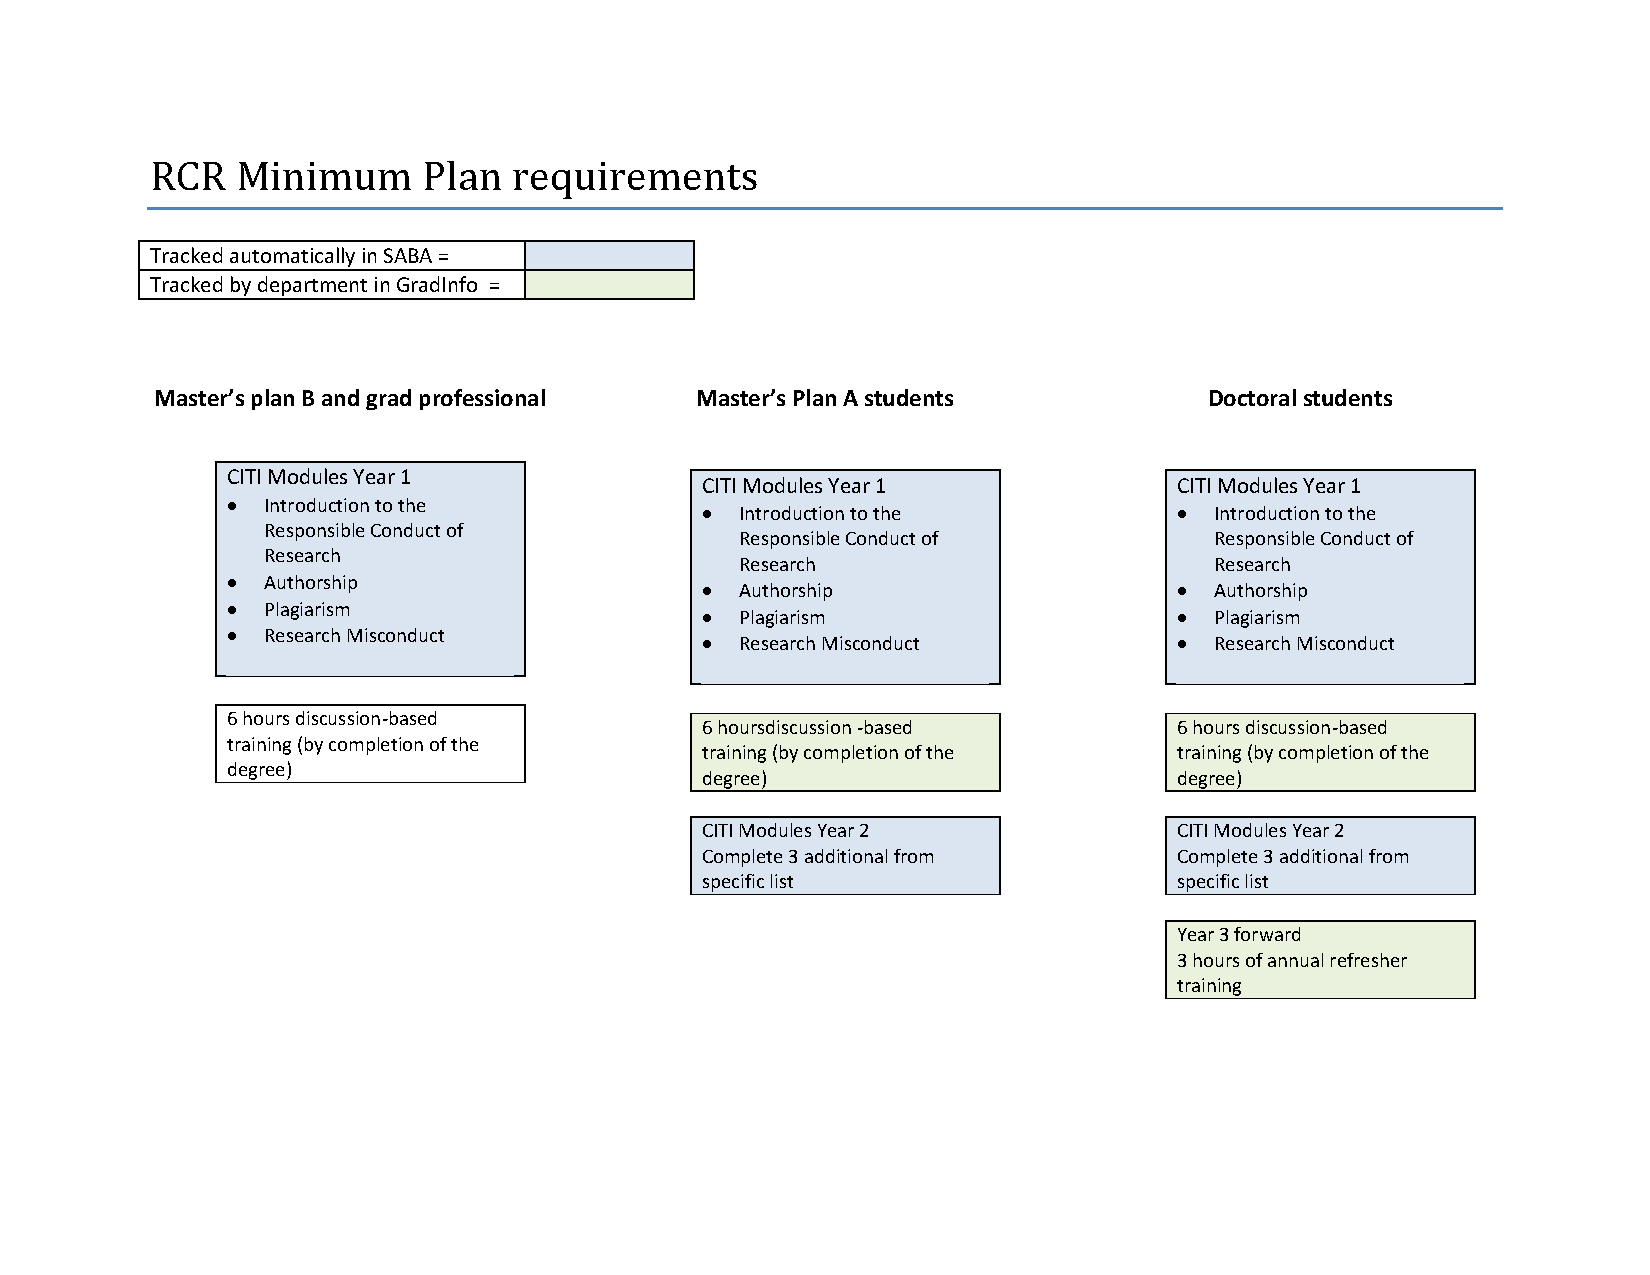
\includegraphics[width=\linewidth]{RCR_minimum_plan_requirements_flow_chart.pdf}
  \caption{RCR minimum plan requirements flow chart.}
  \label{fig:rcr_flowchart}
\end{figure}
\end{center}

\newpage

\section{Examples of dual PhD programs of study}
\label{sec:dual_phd_examples}

This section provides examples of dual PhD programs of study
incorporating CMSE and a second subject for several of the programs
that are common partners in this endeavor.  This information is
provided as guidance for students developing a dual PhD program, and
is non-binding (i.e., it does not represent a set of
\textit{requirements}, simply a set of guidelines).  Final approval of
any dual PhD program rests with the student's dissertation committee
as well as the graduate directors of CMSE and the second PhD program.

The requirements of the CMSE PhD program is described in detail in
Section~\ref{sec:phd}, and the Department of CMSE's guidelines on dual
PhDs with CMSE and a second subject are described in
Section~\ref{sec:dual_phd}.

Note that, regardless of the other department's requirements, the
Department of Computational Mathematics, Science and Engineering
requires that a dual PhD program must form their dissertation
committee (or a guidance committee whose composition approximates
their dissertation committee) prior to the end of their second year in
a MSU PhD program, discuss their planned program of study with this
committee, and ensure that all of the proper paperwork has been
fulfilled by the end of their second year.

%%%%%%%%%%%%%%%%%%%%%%%%%%%%%%%%%%%%%%%%%%%%%%%%%%%%%%%%%%%%%%%%
\subsection{Mathematics}

The mathematics graduate handbook can be
\href{https://mth.msu.edu/graduate/files/handbook/Graduate_Student_Handbook_2015_And_Later.pdf}{found
  here}, and explicitly contains the Department of Mathematics
requirements for a dual PhD in mathematics and a second subject
(section IV.C).

In order to receive a PhD in Mathematics, a student must: (1) satisfy
the qualifying examination requirements by passing written exam
corresponding to 3 of 5 areas of specialization, and taking the
two-semesters course sequences for these areas (18 credits
total), within approximately two years of entrance in the PhD program;
(2) Pass the comprehensive examination in the area of the
student's research interests, which includes both a written and oral
exam; (3) take thirty credits of 800-900 level mathematics courses,
excluding dissertation credits (MTH 999) and core courses in areas in
which the qualifying examination requirements are fulfilled; (4) take
24 dissertation credits (MTH 999); and, (5) write and defend a
doctoral dissertation acceptable to the student's dissertation
committee.

\subsubsection{CMSE as the primary program}

To fulfill the qualifying exam requirements in mathematics, candidates
whose secondary program is mathematics must pass two mathematics
qualifying exams (rather than three) within the first three years of
the student’s enrollment at Michigan State University.  They must pass
three of the CMSE subject exams within their first two years to
fulfill the CMSE qualifying exam requirement.  Students must take 15
credits of 800-900 level mathematics courses, excluding dissertation
credits (Math 999) and qualifying exam course sequences, and must also
take additional computationally-focused courses to satisfy the CMSE
course requirement.  The Department of Mathematics requires that all
candidates with dual PhDs in mathematics must fulfill their
comprehensive examination requirement as specified for PhD candidates
in mathematics, any time after the qualifying exam requirements have
been met and prior to the end of the student's fourth year at MSU.
Furthermore, the comprehensive exam can include topics and questions
from the dual program to allow the comprehensive exam to satisfy the
requirements of the dual program, although at least half the topics
and questions should be in mathematics.  A further restriction is that
the topics covered by the comprehensive exam must be approved by the
Mathematics graduate director and Mathematics graduate studies
committee.  To  satisfy the CMSE comprehensive exam
requirements, students must write a comprehensive exam paper
containing the same material as a student fully within the CMSE PhD
program, as described in Section~\ref{sec:comp_exam}.  Regarding
committee members, the Mathematics requirement is as follows: ``For
secondary candidates the guidance committee and dissertation committee
should consist of four or more tenure stream faculty members at least
40\% of whom have a 50\% or more appointment in Mathematics.''  The
Department of CMSE requires that at least one faculty member have
their tenure home in CMSE (i.e., more than 50\% of their appointment
in CMSE).  Dissertation credits should be in CMSE (i.e., CMSE 999).


\subsubsection{Mathematics as the primary program}

According to the Mathematics guidelines, students pursuing a dual PhD
with mathematics as the primary program must fulfill the qualifying
course and exams requirements exactly as specified for PhD candidates
in mathematics and in the same time frame.  In addition, these
students must pass two of the CMSE subject exams within their first
two years.  Students must take 21 credits of 800-900 level mathematics
courses, excluding dissertation credits (Math 999) and qualifying exam
course sequences.  Students must take a minimum of 15 credits of
coursework in computationally-focused subjects to satisfy their CMSE
course requirements, which may be satisfied by computationally-focused
mathematics courses.
The Department of Mathematics requires that all candidates with dual
PhDs in mathematics must fulfill their comprehensive examination
requirement as specified for PhD candidates in mathematics, any time
after the qualifying exam requirements have been met and prior to the
end of the student's fourth year at MSU.  Furthermore, the
comprehensive exam can include topics and questions from the dual
program to allow the comprehensive exam to satisfy the requirements of
the dual program, although at least half the topics and questions
should be in mathematics.  A further restriction is that the topics
covered by the comprehensive exam must be approved by the Mathematics
graduate director and Mathematics graduate studies committee.  To
satisfy the CMSE comprehensive exam requirements, students must write
a comprehensive exam paper containing the same material as a student
fully within the CMSE PhD program, as described in
Section~\ref{sec:comp_exam}.  Regarding committee members, the
Mathematics requirement is as follows: ``For primary candidates the
guidance committee and dissertation committee should consist of four
or more tenure stream faculty members at least half of whom have a
50\% or more appointment in Mathematics.''  The Department of CMSE
requires that at least one faculty member have their tenure home in
CMSE (i.e., more than 50\% of their appointment in CMSE).
Dissertation credits should be in Mathematics (i.e., MTH 999).


%%%%%%%%%%%%%%%%%%%%%%%%%%%%%%%%%%%%%%%%%%%%%%%%%%%%%%%%%%%%%%%%
\subsection{Statistics and Probability}

Information on the Statistics PhD program can be
\href{https://www.stt.msu.edu/Graduate_Program/handbook/PHDREQ.pdf}{found
  here}.

In order to receive a PhD in Statistics and Probability, a student
must (1) take the 5 core STT courses (STT 872, 881-2, 867-8; 15
credits total), (2) take at least 5 courses in advanced probability or
statistics, with at least one in each category (15 credits), (3) take
3 elective courses (9 credits), which may be from outside the
department, (4) pass the Probability and Statistics preliminary
examinations within three years of being admitted to the program, and
(5) complete an original dissertation and enroll in at least 24
credits of STT 999.  The PhD program in Statistics and Probability has
no comprehensive exam requirement.

\subsubsection{CMSE as the primary program}

Students pursuing a dual PhD with CMSE as the primary program must
take STT 87 and 881, as well as any three of the four core CMSE
courses (CMSE 820-823).  They must pass one of the Statistics
preliminary exams and at least thre of the CMSE subject exams.  They
must further take 5 elective courses, with at least 2 from STT (with
the STT courses chosen from the remaining core STT and/or advanced
probability and statistics courses, and CMSE requirements as specified
elsewhere in this handbook).  Students must take the CMSE
comprehensive examination.  No particular requirements are specified
regarding guidance committee composition; however, at least one member
of the committee must have their tenure home in each of the two
departments.

\subsubsection{Statistics as the primary program}

Students pursuing a dual PhD with statistics as the primary program
must take STT 872, 881, and one course selected from STT 882, 867,
868, as well as any two of the four core CMSE courses (CMSE 820-823).
They must pass at least one of the Statistics preliminary exams and at
least two of the CMSE subject exams.  They must further take 5
elective courses, with at least 3 from STT (with the STT courses
chosen from the remaining core STT and/or advanced probability and
statistics courses, and CMSE requirements as specified elsewhere in
this handbook).  Students must take a minimum of 15 credits of
coursework in computationally-focused subjects to satisfy their CMSE
course requirements, which may be satisfied by computationally-focused
statistics courses.  Students must take the CMSE comprehensive
examination.  No particular requirements are specified regarding
guidance committee composition; however, at least one member of the
committee must have their tenure home in each of the two departments.


%%%%%%%%%%%%%%%%%%%%%%%%%%%%%%%%%%%%%%%%%%%%%%%%%%%%%%%%%%%%%%%%
\subsection{Physics}

The Physics and Astrophysics graduate handbook can be \href{http://www.pa.msu.edu/grad/GradHandbook.pdf}{found
  here}.  
To receive a PhD in physics, students must: (1) pass the physics
qualifying examination, (2) complete a set of 7 core physics courses
(PHY 810, 820, 831, 851-2, 841-2), (3) fulfill the comprehensive exam
requirement by receiving acceptable grades in the subject exams
associated with PHY 820, 831, 841, and 851-2, (4) complete an original
dissertation and enroll in at least 24 credits of PHY 999, and (5)
serve as a Teaching Assistant (TA) for at least one semester.

\subsubsection{CMSE as the primary program}

Students pursuing a dual PhD with CMSE as the primary program must
take 3 of the 4 core CMSE courses and pass the corresponding subject
exams and take 2 of the 4 core PHY courses (or course sequences) and
pass the corresponding subject exams.  The remainder of the student's
coursework requirement can be fulfilled by any reasonable combination
of PHY and CMSE coursework, with students strongly advised to take
additional physics courses.  Students must take the CMSE comprehensive
examination.  The dissertation committee consists of five members with
at least two having their tenure homes in the Physics and Astronomy
department (with no requirement as to the members' sub-discipline) and
at least one member having their tenure home in CMSE.  Students with
CMSE as their primary program do not have a requirement that they
serve as a teaching assistant.  These students should take CMSE
dissertation credits (CMSE 999).

\subsubsection{Physics as the primary program}

Students pursuing a dual PhD with Physics as the primary program must
take 3 of the 4 core PHY courses (or course sequences) and pass the
corresponding subject exams and take 2 of the 4 core CMSE courses and
pass the corresponding subject exams.  The remainder of the student's
coursework requirement can be fulfilled by any reasonable combination
of PHY and CMSE coursework, with students strongly advised to take
significant additional physics courses.  Students must take a minimum
of 15 credits of coursework in computationally-focused subjects to
satisfy their CMSE course requirements, which may be satisfied by
computationally-focused physics courses.  Students must take the CMSE
comprehensive examination.  The dissertation committee consists of
five members with at least three having their tenure homes in the
Physics and Astronomy department (with one being from outside the
student's interest area) and at least one member having their tenure
home in CMSE.  These students should take Physics dissertation credits
(PHY 999).

%%%%%%%%%%%%%%%%%%%%%%%%%%%%%%%%%%%%%%%%%%%%%%%%%%%%%%%%%%%%%%%%
\subsection{Astrophysics}

The Physics and Astrophysics graduate handbook can be \href{http://www.pa.msu.edu/grad/GradHandbook.pdf}{found
  here}.  

To receive a PhD in astrophysics, students must take a total of eight
courses comprising the four core astronomy courses (AST 810, AST 825,
AST 835, and AST 840), two of the physics subject exam courses
(PHY820, PHY 831, PHY 841, and PHY 851), and two additional courses (6
credits) selected from the core physics, astrophysics, or
computational courses.  Furthermore, they must complete an original
dissertation and enroll in at least 24 credits of PHYAST 999, and
serve as a Teaching Assistant (TA) for at least one semester.

\subsubsection{CMSE as the primary program}

Students pursuing a dual PhD with CMSE as the primary program must
take 3 of the 4 core CMSE courses and pass the corresponding subject
exams and take 2 of the 4 core AST courses (or course sequences) and
pass the corresponding subject exams.  The remainder of the student's
coursework requirement can be fulfilled by any reasonable combination
of AST, PHY, and CMSE coursework, with students strongly advised to
take at least one of the physics courses.  Students must take the CMSE
comprehensive examination.  The dissertation committee consists of
five members with at least two having their tenure homes in the
Physics and Astronomy department (with no requirement as to the
members' sub-discipline) and at least one member having their tenure
home in CMSE.  Students with CMSE as their primary program do not have
a requirement that they serve as a teaching assistant.  These students
should take CMSE dissertation credits (CMSE 999).

\subsubsection{Astrophysics as the primary program}

Students pursuing a dual PhD with Astrophysics as the primary program
must take 3 of the 4 core AST courses and take 2 of the 4 core CMSE
courses and pass the corresponding subject exams.  The remainder of
the student's coursework requirement can be fulfilled by any
reasonable combination of AST, PHY, and CMSE coursework, with students
strongly advised to take at least one of the physics courses.
Students must take the CMSE comprehensive examination.  The
dissertation committee consists of five members with at least three
having their tenure homes in the Physics and Astronomy department
(with one being from outside the student's interest area) and at least
one member having their tenure home in CMSE.  These students should
take Astrophysics dissertation credits (AST 999).



\end{document}
